%% bare_conf_compsoc.tex
%% V1.4b
%% 2015/08/26
%% by Michael Shell
%% See:
%% http://www.michaelshell.org/
%% for current contact information.
%%
%% This is a skeleton file demonstrating the use of IEEEtran.cls
%% (requires IEEEtran.cls version 1.8b or later) with an IEEE Computer
%% Society conference paper.
%%
%% Support sites:
%% http://www.michaelshell.org/tex/ieeetran/
%% http://www.ctan.org/pkg/ieeetran
%% and
%% http://www.ieee.org/

%%*************************************************************************
%% Legal Notice:
%% This code is offered as-is without any warranty either expressed or
%% implied; without even the implied warranty of MERCHANTABILITY or
%% FITNESS FOR A PARTICULAR PURPOSE! 
%% User assumes all risk.
%% In no event shall the IEEE or any contributor to this code be liable for
%% any damages or losses, including, but not limited to, incidental,
%% consequential, or any other damages, resulting from the use or misuse
%% of any information contained here.
%%
%% All comments are the opinions of their respective authors and are not
%% necessarily endorsed by the IEEE.
%%
%% This work is distributed under the LaTeX Project Public License (LPPL)
%% ( http://www.latex-project.org/ ) version 1.3, and may be freely used,
%% distributed and modified. A copy of the LPPL, version 1.3, is included
%% in the base LaTeX documentation of all distributions of LaTeX released
%% 2003/12/01 or later.
%% Retain all contribution notices and credits.
%% ** Modified files should be clearly indicated as such, including  **
%% ** renaming them and changing author support contact information. **
%%*************************************************************************


% *** Authors should verify (and, if needed, correct) their LaTeX system  ***
% *** with the testflow diagnostic prior to trusting their LaTeX platform ***
% *** with production work. The IEEE's font choices and paper sizes can   ***
% *** trigger bugs that do not appear when using other class files.       ***                          ***
% The testflow support page is at:
% http://www.michaelshell.org/tex/testflow/



\documentclass[conference,compsoc]{IEEEtran}
% Some/most Computer Society conferences require the compsoc mode option,
% but others may want the standard conference format.
%
% If IEEEtran.cls has not been installed into the LaTeX system files,
% manually specify the path to it like:
% \documentclass[conference,compsoc]{../sty/IEEEtran}
% *** MISC UTILITY PACKAGES ***
%
%\usepackage{ifpdf}
% Heiko Oberdiek's ifpdf.sty is very useful if you need conditional
% compilation based on whether the output is pdf or dvi.
% usage:
% \ifpdf
%   % pdf code
% \else
%   % dvi code
% \fi
% The latest version of ifpdf.sty can be obtained from:
% http://www.ctan.org/pkg/ifpdf
% Also, note that IEEEtran.cls V1.7 and later provides a builtin
% \ifCLASSINFOpdf conditional that works the same way.
% When switching from latex to pdflatex and vice-versa, the compiler may
% have to be run twice to clear warning/error messages.






% *** CITATION PACKAGES ***
%
\ifCLASSOPTIONcompsoc
  % IEEE Computer Society needs nocompress option
  % requires cite.sty v4.0 or later (November 2003)
  \usepackage[nocompress]{cite}
\else
  % normal IEEE
  \usepackage{cite}
\fi

\ifCLASSINFOpdf
  \usepackage[pdftex]{graphicx}
  % declare the path(s) where your graphic files are
  % \graphicspath{{../pdf/}{../jpeg/}}
  % and their extensions so you won't have to specify these with
  % every instance of \includegraphics
  % \DeclareGraphicsExtensions{.pdf,.jpeg,.png}
\else
  % or other class option (dvipsone, dvipdf, if not using dvips). graphicx
  % will default to the driver specified in the system graphics.cfg if no
  % driver is specified.
  % \usepackage[dvips]{graphicx}
  % declare the path(s) where your graphic files are
  % \graphicspath{{../eps/}}
  % and their extensions so you won't have to specify these with
  % every instance of \includegraphics
  % \DeclareGraphicsExtensions{.eps}
\fi

\usepackage{amsmath}
\usepackage{algorithm}
\usepackage{algorithmic}
\usepackage{array}

% *** SUBFIGURE PACKAGES ***
% \ifCLASSOPTIONcompsoc
%  \usepackage[caption=false,font=footnotesize,labelfont=sf,textfont=sf]{subfig}
% \else
%  \usepackage[caption=false,font=footnotesize]{subfig}
% \fi
% subfig.sty, written by Steven Douglas Cochran, is the modern replacement
% for subfigure.sty, the latter of which is no longer maintained and is
% incompatible with some LaTeX packages including fixltx2e. However,
% subfig.sty requires and automatically loads Axel Sommerfeldt's caption.sty
% which will override IEEEtran.cls' handling of captions and this will result
% in non-IEEE style figure/table captions. To prevent this problem, be sure
% and invoke subfig.sty's "caption=false" package option (available since
% subfig.sty version 1.3, 2005/06/28) as this is will preserve IEEEtran.cls
% handling of captions.
% Note that the Computer Society format requires a sans serif font rather
% than the serif font used in traditional IEEE formatting and thus the need
% to invoke different subfig.sty package options depending on whether
% compsoc mode has been enabled.
%
% The latest version and documentation of subfig.sty can be obtained at:
% http://www.ctan.org/pkg/subfig


\usepackage{url}
\usepackage{amsfonts}  
\usepackage{latexsym}  
\usepackage{amsmath, mathtools}  
\usepackage{bbm}
\usepackage{fancybox}  
%\usepackage{times}  
\usepackage{color}
%\usepackage{lscape}  
\usepackage{enumitem}
\usepackage{caption}
\usepackage{subcaption}
\usepackage{hyperref}

% \usepackage{subfigure}
% correct bad hyphenation here
\hyphenation{op-tical net-works semi-conduc-tor}
\newcommand{\bS}{\bm{S}}
\newcommand{\mE}{\mathbb{E}}
\newcommand{\mR}{\mathbb{R}}
\newcommand{\Paux}{P_{\textrm{aux}}}
\newcommand{\Pcase}{P_{\textrm{case}}}

\newcommand{\hub}{\emph{The Hub}}
\newcommand{\ar}{AR}
\newcommand{\sar}{AR\_spatial}
\newcommand{\aacomment}[1]{({\color{red}AA: #1})}
\newcommand{\blcomment}[1]{({\color{green}BL: #1})}
\newcommand{\svcomment}[1]{({\color{magenta}SV: #1})}
\newcommand{\bhcomment}[1]{({\color{blue}BH: #1})}
\newcommand{\mmcomment}[1]{({\color{purple}MM: #1})}
\newcommand{\gkcomment}[1]{({\color{orange}GK: #1})}
\newcommand{\lwcomment}[1]{({\color{pink}LW: #1})}

\begin{document}
%
% paper title
% Titles are generally capitalized except for words such as a, an, and, as,
% at, but, by, for, in, nor, of, on, or, the, to and up, which are usually
% not capitalized unless they are the first or last word of the title.
% Linebreaks \\ can be used within to get better formatting as desired.
% Do not put math or special symbols in the title.
\title{Enhancing COVID-19 Ensemble Forecasting Model Performance Using Auxiliary Data Sources}
% \title{Phase-informed Bayesian Ensemble Training}

% author names and affiliations
% use a multiple column layout for up to three different
% affiliations
\author{\IEEEauthorblockN{Aniruddha Adiga\IEEEauthorrefmark{1}\textsuperscript{\textsection}, Gursharn Kaur\IEEEauthorrefmark{1}\textsuperscript{\textsection}, Benjamin Hurt\IEEEauthorrefmark{1}, Lijing Wang\IEEEauthorrefmark{2}, Przemyslaw Porebski\IEEEauthorrefmark{1}, \\ Srinivasan Venkatramanan\IEEEauthorrefmark{1}, Bryan Lewis\IEEEauthorrefmark{1}, Madhav Marathe\IEEEauthorrefmark{1}\IEEEauthorrefmark{3}}
\IEEEauthorblockA{\IEEEauthorrefmark{1}Biocomplexity Institute,
University of Virginia, Charlottesville, Virginia}
\IEEEauthorblockB{\IEEEauthorrefmark{2} New Jersey Institute of Technology, Newark, New Jersey}\\
\IEEEauthorblockB{\IEEEauthorrefmark{3}Dept. of Computer Science,
University of Virginia,
Charlottesville, Virginia\\
Email: aniruddha@virginia.edu, marathe@virginia.edu}}
% \and
% \IEEEauthorblockN{Homer Simpson}
% \IEEEauthorblockA{Twentieth Century Fox\\
% Springfield, USA\\
% Email: homer@thesimpsons.com}
% \and
% \IEEEauthorblockN{James Kirk\\ and Montgomery Scott}
% \IEEEauthorblockA{Starfleet Academy\\
% San Francisco, California 96678-2391\\
% Telephone: (800) 555--1212\\
% Fax: (888) 555--1212}}
% conference papers do not typically use \thanks and this command
% is locked out in conference mode. If really needed, such as for
% the acknowledgment of grants, issue a \IEEEoverridecommandlockouts
% after \documentclass

% for over three affiliations, or if they all won't fit within the width
% of the page (and note that there is less available width in this regard for
% compsoc conferences compared to traditional conferences), use this
% alternative format:
% 
%\author{\IEEEauthorblockN{Michael Shell\IEEEauthorrefmark{1},
%Homer Simpson\IEEEauthorrefmark{2},
%James Kirk\IEEEauthorrefmark{3}, 
%Montgomery Scott\IEEEauthorrefmark{3} and
%Eldon Tyrell\IEEEauthorrefmark{4}}
%\IEEEauthorblockA{\IEEEauthorrefmark{1}School of Electrical and Computer Engineering\\
%Georgia Institute of Technology,
%Atlanta, Georgia 30332--0250\\ Email: see http://www.michaelshell.org/contact.html}
%\IEEEauthorblockA{\IEEEauthorrefmark{2}Twentieth Century Fox, Springfield, USA\\
%Email: homer@thesimpsons.com}
%\IEEEauthorblockA{\IEEEauthorrefmark{3}Starfleet Academy, San Francisco, California 96678-2391\\
%Telephone: (800) 555--1212, Fax: (888) 555--1212}
%\IEEEauthorblockA{\IEEEauthorrefmark{4}Tyrell Inc., 123 Replicant Street, Los Angeles, California 90210--4321}}




% use for special paper notices
%\IEEEspecialpapernotice{(Invited Paper)}




% make the title area
\maketitle
\begingroup\renewcommand\thefootnote{\textsection}
\footnotetext{Equal contribution}
\endgroup

% As a general rule, do not put math, special symbols or citations
% in the abstract
\begin{abstract}
Real-time forecasting of non-stationary time series is a challenging problem,  especially when the time series evolves rapidly. For such cases, it has been observed that ensemble models consisting of a diverse set of model classes can perform consistently better than individual models. In order to account for the nonstationarity of the data and the lack of availability of training examples, the models are retrained in real-time using the most recent observed data samples. Motivated by the robust performance properties of ensemble models, we developed a Bayesian model averaging ensemble technique consisting of statistical, deep learning, and compartmental models for forecasting epidemiological signals, specifically, COVID-19 signals. We observed the epidemic dynamics go through several phases (waves). In our ensemble model, we observed that different model classes performed differently during the various phases. Armed with this understanding, in this paper, we propose a modification to the ensembling method to employ this phase information and use different weighting schemes for each phase to produce improved forecasts. However, predicting the phases of such time series is a significant challenge, especially when behavioral and immunological adaptations govern the evolution of the time series. We explore multiple datasets that can serve as leading indicators of trend changes and employ \emph{transfer entropy} techniques to capture the relevant indicator. We propose a phase prediction algorithm to estimate the phases using the leading indicators. Using the knowledge of the estimated phase, we selectively sample the training data from similar phases. We evaluate our proposed methodology on our currently deployed COVID-19 forecasting model and the COVID-19 ForecastHub models. The overall performance of the proposed model is consistent across the pandemic. More importantly, it is ranked \emph{second} during two critical rapid growth phases in cases, regimes where the performance of most models from the ForecastHub dropped significantly.     

% Ensembling methods that can employ these phase information and use different weighting schemes for each phase can produce improved forecasts. 


% Despite hundreds of methods published in the literature, forecasting epidemic dynamics continues to be a challenging yet important problem. The challenges stem from multiple sources, including: lack of timely data, co-evolution of epidemic dynamics with behavioral and immunological adaptations, and the evolution of new pathogen strains. The ongoing COVID-19 pandemic highlighted these challenges; in an important article, Reich et al. did a comprehensive analysis highlighting many of these challenges.

% In this paper, we take another step in critically evaluating existing epidemic forecasting methods. Armed with this understanding, we propose a modification to our deployed Bayesian ensembling case time series forecasting framework to combine existing methods and produce a composite forecast. Our methods are based on a simple yet crucial observation --- epidemic dynamics go through a number of phases (waves). Ensembling methods that can employ these phase information and use different weighting schemes for each phase can produce improved forecasts. 
% %This is in contrast to improving the individual models which are then fed into an ensemble model.
% We evaluate our proposed method with both the currently deployed model and the COVID-19 forecasthub models. The overall performance of the proposed model is consistent across the pandemic but more importantly, it is ranked \emph{third} and \emph{first} during two critical rapid growth phases in cases, regimes where the performance of most models from CDC forecasting hub dropped significantly.

\end{abstract}

% no keywords




% For peer review papers, you can put extra information on the cover
% page as needed:
% \ifCLASSOPTIONpeerreview
% \begin{center} \bfseries EDICS Category: 3-BBND \end{center}
% \fi
%
% For peerreview papers, this IEEEtran command inserts a page break and
% creates the second title. It will be ignored for other modes.
\IEEEpeerreviewmaketitle



\section{Introduction}
An ensemble of models have been studied extensively and have shown to produce superior performance when compared to individual models~\cite{sagi2018ensemble}. In forecasting, ensemble models, specifically, Bayesian model averaging (BMA)~\cite{raftery2005using} which are suitable for ensembling probabilistic forecasts have been shown to produce superior performance over individual models in varied applications such as  epidemilogy~\cite{yamana2016superensemble,reich2019collaborative,cramer2022evaluation}, weather predictions~\cite{raftery2005using}, hydrology~\cite{duan2007multi}, political sciences~\cite{montgomery2012improving}, etc. Given, its wide-spread use in probabilistic forecasting, we developed a multi-class BMA ensemble model for COVID-19 case forecasting~\cite{allmodels} in order to provide weekly forecasts to the CDC's COVID-19 ForecastHub (also referred to as \hub{})~\cite{Cramer2021-hub-dataset}. We are one of
the teams contributing forecasts (listed as \textsc{UVA-Ensemble}) since July 2020 and focused on incident cases and hospitalizations at a granular level. The constituent models in the \textsc{UVA-Ensemble} forecasting method include several standard statistical, deep learning and compartmental models. Specifically, we employ autoregressive models and its variants (AR with spatial exogenous regressor, ARIMA), an LSTM model, an ensemble Kalman filter (EnKF), and a compartmental model (SEIR). A detailed description of the models is available in our work~\cite{allmodels}.In order to account for nonstationarity of the case time series, we retrain the models every week.  

 An ensemble model, despite providing robust performances, is dependent on the quality of its constituent models. Despite the efforts of the forecasting community, there is considerable lack of understanding of disease dynamics as teams have struggled to predict the onset, growth rate, peak size, and duration of the various waves. Achieving good forecasting accuracy during the growth or surge phase is of high importance as it enables effective allocation of medical resources which are strained during these times. Hence, the ensemble models have suffered from outlying forecasts and have failed to catch the local peaks~\cite{ray2021challenges}, a trend we have also observed in our own ensemble model forecasts. 
 \\
\textbf{Key observations from our real-time forecasting effort}
\begin{itemize}
    \item In the COVID-19 cases time series, we observe three distinct phases characterized by periods of rapid growth, plateau, and steady decline. The rapid growth phases are particularly critical as they often lead to severe burden on the medical resources.
    \item An ensemble model, despite providing robust performances, is dependent on the quality of its constituent models. Despite the best effort of the modelers, due to a lack of understanding of the disease dynamics of the novel virus, most teams struggled to forecast the waves, including our models. 
    \item A retrospective evaluation of our deployed model \cite{allmodels} in \hub{} across the forecasting weeks indicates that the BMA has a performance close to \hub's ensemble model. Further, we performed model ablation analysis to understand the influence of individual models on the ensemble. Our analysis indicates that: ($i$) compartmental models are useful during growth and decline phases but tend to over-predict during surge and decline phases; ($ii$) purely data-driven models like LSTMs have a latency in picking up the change in phases, but can quickly learn the patterns and ($iii$) Statistical AR methods or Kalman filters based methods show superior performance during time of relative steady phase of the pandemic.
    
\end{itemize}

These observations have prompted us to modify the ensemble model to incorporate the phase information in the training and propose a phase-informed BMA model. These new methods employ big data analytics and machine learning techniques such as transfer entropy~\cite{schreiber2000measuring} to improve on forecasting performance. The contribution of this paper is three fold and is summarized as follows:
\subsection{Summary of contributions.}
\noindent
\textbf{Development of a new phase-informed BMA.}
We propose a modification to the BMA training where only training samples corresponding to a particular phase are employed to determine the weights. This selective sampling helps influence the BMA to assign higher weights to models with superior performance during similar phases observed historically. 
\\
\textbf{Identifying leading indicators from multiple data sources}
In the phase prediction, a major challenge is to determine leading indicators to the case time series. We propose a transfer entropy technique~\cite{schreiber2000measuring} to obtain the leading indicators and then predict the phase for the target time series as a function of the phases of the leading indicators (sources). 
\\
\textbf{Phase inference}
We present a new, simple method to address the problem of phase classification of a given time series. The phase classification involves assigning each time point to one of three phases \{\emph{Surge}, \emph{Plateau}, \emph{Decline}\}. This is achieved by approximating the time series as a piece-wise linear signal and then inferring the phase based on the slope the linear fits. 
\\
Using the phase information, the BMA model is able to leverage the context-specific historical performance of individual methods thus leading to improved forecast performance of the ensemble at critical phases. 
Although, we analyze the efficacy of the proposed training method using our BMA model, the training scheme is fairly generic and can be applied to real-time forecasting tasks, for example to the likes of COVID-19 Forecasthub ensemble models.


An outline of the steps included in the pipeline is given in Figure~\ref{fig:pipeline}.
\begin{figure*}[!t]
    \centering
    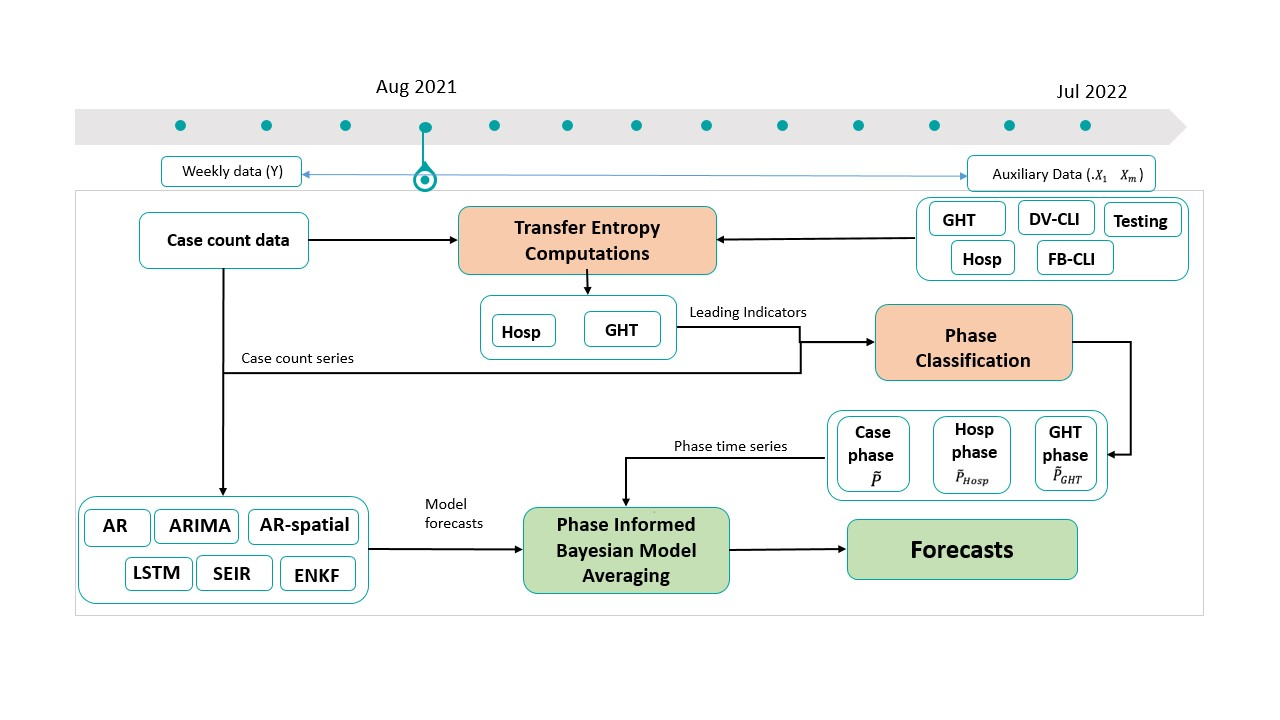
\includegraphics[width=0.99\textwidth]{figs/flow-diagram.jpeg}
    \caption{Workflow of the proposed phase-informed BMA}
    \label{fig:pipeline}
\end{figure*}


% \subsection{Summary of contributions.} 
% \emph{Development of new phase-informed BMA.(Section~\ref{sec:PIBMA})} \
% Based on the phase predictions obtained from auxiliary data sources, we propose an improvement to our BMA model training technique. We modify our ensembling technique to employ training data from historically similar phases as predicted phase. \textbf{We carry out detailed retrospective analysis to show that the new methods lead to improved performance at a critical phase, the surge phase, when compared to existing methods. Our analysis shows that the proposed model has consistent performance across the pandemic. More importantly, it performs significantly well when compared to the \hub{} models during the Delta wave's surge period (median ranking of 3) and Omicron wave's surge phase (median ranking of 1), regime where the performance of most models from the CDC forecasting hub dropped significantly} 

% \paragraph 
% \noindent
% \textbf{Summary of contributions.} \ In this paper, we take a critical look at our state-of-the-art forecasting methods developed and deployed during the ongoing pandemic~\cite{allmodels} and propose new methods based 
% on the insights obtained as a result of our analysis. These new methods employ popular big data and artificial intelligence techniques such as transfer entropy and ensembling methods. Our contributions consists of two key components:


% \noindent
% \emph{Phase prediction using multiple data sources  (Section~\ref{sec:retro}).}  \
% As described previously, the COVID-19 cases time series is characterized by periods of rapid growth, plateau, and steady decline and the individual models in the ensemble have shown variable performance during these phases. Hence forecasting these  phases becomes important as it can used to guide the ensemble to employ training samples from the appropriate phase. Several auxiliary signals exist but it is important to chose only the leading indicators. Since the auxiliary signals and the case time are acquired from different complex reporting systems they often exhibit nonlinear relationships. Hence, we employ transfer entropy, a model-free approach that computes the conditional mutual information between the source and the target, to determine information flow between them. Once, we determine the leading indicators, we classify them into phases and employ their current phase to forecast the phase of the cases time series.      

% \noindent
% \emph{Development of new phase-informed methods.(Section~\ref{sec:PIBMA})} \
% Based on the phase predictions obtained from auxiliary data sources, we propose an improvement to our BMA model training technique. We modify our ensembling technique to employ training data from historically similar phases as predicted phase. \textbf{We carry out detailed retrospective analysis to show that the new methods lead to improved performance at a critical phase, the surge phase, when compared to existing methods. Our analysis shows that the proposed model has consistent performance across the pandemic. More importantly, it performs significantly well when compared to the \hub{} models during the Delta wave's surge period (median ranking of 3) and Omicron wave's surge phase (median ranking of 1), regime where the performance of most models from the CDC forecasting hub dropped significantly}

\subsection{Related Works}
% \section{Auxiliary Data Sources and Integration using Transfer Entropy}
In the context of epidemic forecasting, auxiliary data sources have been employed extensively for improving forecast accuracy. 
In influenza-like illness and dengue forecasting additional sources such as Google health search trends, medical health records, weather data have been extensively s in forecasting models have shown to improve forecasting accuracy~\cite{yang2015accurate, prashant2019PLOSCompBio,shaman2012forecasting}. Similarly, in COVID-19 forecasting, mobility data, digital thermometers, medical records, etc. ~\cite{kapoor2020examining,wang2020using,fritz2021combining,rodriguez2020deepcovid}. 
The COVIDcast~\cite{reinhart2021open} data repository, has been able to aggregate data from mulitple providers and Faceook surveys. The utility of the dataset in forecasting is discussed in~\cite{mcdonald2021can}.  

Multiple measures exist for determining the information flow between two signals, a popular method is the Granger causality test~\cite{granger1969investigating} which determines the linear relationship between signals, which is rarely the case. Under such circumstances the use information theoretic approaches such as transfer entropy~\cite{schreiber2000measuring}, mutual information~\cite{dionisio2004mutual} and symbolic transfer entropy~\cite{staniek2008symbolic} have been shown to capture the source-target information flows.

\section{Phase-Informed Bayesian Model Averaging}\label{sec:PIBMA}
Motivated by the observation that certain models perform better during certain \emph{phases}, we propose a method to supply the phase information during the BMA ensemble training. In the BMA framework, we train independently, one model per location. Considering $K$ models per location, the BMA assumes that the conditional density of observing case count $y$ given the forecasts $f_1, \dots, f_K$ generated from  models $M_1, M_2, \dots, M_K$ is given by 
\begin{equation}
    p(y| f_1, f_2, \cdots, f_K) = \sum_{k=1}^{K} w_k g_k (y|f_k),
    \label{eq:bma_pdf}
\end{equation}
where $w_k$ is the posterior probability of the $k^{\mathrm{th}}$ model's forecast being the best one and $g_k(y|f_k)$ is the conditional density of $y$ given $f_k$. With normal approximation for the conditional density i.e. $y|f_k \sim \mathcal{N}(f_k,\sigma^2_k)$, \eqref{eq:bma_pdf} is a finite mixture of Gaussians and we proceed to determine the weights $w_k$ and $\sigma_k$. Given the distribution \eqref{eq:bma_pdf}, the weights and variance parameters are obtained as the maximum likelihood estimate using the standard expectation-maximization (EM) algorithm \cite{raftery2005using}, which
%The resulting log-likelihood function does not have an analytical solution, and the estimates are obtained using the standard expectation-maximization (EM) algorithm \cite{raftery2005using,yamana2017individual}. Given $\mathcal{\tau}$ training samples, the optimization procedure
alternates between the E-step and the M-step with the updates for $w_k$ and $\sigma_k$ in the $j^{\text{th}}$ iteration given by the (E-step)
\begin{align}
% \footnotesize
    \quad z^{(j)}_{k,t} = \frac{w^{(j-1)}_kg({y_t|f_{k,t}, \sigma_k^{(j-1)}})}{\sum_{i=1}^K w^{(j-1)}_i g(y_t|f_{i,t}, \sigma_i^{(j-1)})}, \nonumber\\ \intertext{and (M-step)}
     w^{(j)}_k = \frac{1}{|\mathcal{T}|} \sum_{t \in \mathcal{T}} z_{k,t}^{(j)}, \; \sigma^{(j)2}_k = \frac{\sum_{t \in \mathcal{T}}z_{k,t}(y_t-f_{k,t})^2}{\sum_{t \in \mathcal{T}}z_{k,t}  }.
    \label{eq:bma_fixed}
\end{align}

 In the existing framework \cite{allmodels}, $\mathcal{T}$ corresponds to the previous $N$ contiguous weeks of training samples, that is, for a forecast week $T$, $\mathcal{T}=\{T-1, T-2, \cdots, T-N\}$. Given the highly nonstationary data, in order to ensure that the most recent trend is captured, we consider only the most recent N weeks of performance in the training and not the entire set of historical forecasts. 

  Since the weights are estimated based on the individual model performances over the past $N$ weeks, this introduces a latency in picking the best model during a phase change. The model has to observe sufficient forecasts from the best performing model over the next few weeks to put higher weights on it. This latency leads to the BMA model to produce under-performing forecasts.
 
We identify and address this issue by designing a BMA ensemble that uses the knowledge of the relevant phase to get improved forecasts. On that note, for a weekly case counts time series, we first segment the ground truth week indices into surge (S), decline (D), and plateau (P) phases. Let $\mathcal{T}_S$, $\mathcal{T}_D$, and $\mathcal{T}_P$ be the set of all week indices corresponding to the surge, decline, and plateau, respectively. The phase-informed BMA then considers all the historical forecasts made by individual methods during the specified phase for training the weights. That is, for a particular phase $r \in \{S,D,P\}$, estimation of weights and variance in \eqref{eq:bma_fixed} (M-Step) can be modified as
\begin{eqnarray}
    w^{(j)}_{k,r} = \frac{1}{|\mathcal{T}_r|} \sum_{t \in \mathcal{T}_r} z_{k,t}^{(j)}, \;
    \sigma^{(j)2}_{k,r} = \frac{\sum_{t \in \mathcal{T}_r}z_{k,t}(y_t-f_{k,t})^2}{\sum_{t \in \mathcal{T}_r}z_{k,t}  }.
\end{eqnarray}
We next discuss the phase prediction technique that enables us to determine $\mathcal{T}_r$.
\subsection{Transfer Entropy for Identifying Leading Indicators} \label{subsec:phase.pred}

\subsubsection{Data Sources} \label{sec:data-src}
Since early 2020, \cite{covidcast} has collaborated with data partners to collect, curate, and make publicly available numerous real-time spatio-temporal COVID-19 indicators. These indicators have been aggregated to provide multiple views of pandemic activity in the United States~\cite{reinhart2021open}. Some of the data sources have been shown to be leading indicators of the case time series~\cite{mcdonald2021can}. Additionally, these indicators are available at multiple resolutions (example at state level, county level, etc.). In this paper we consider signals only at the state-level as the reporting has been relatively consistent and less noisy compared to county-level signals.


% Assuming we have $K$ indicators for every location $\ell$, we denote the set of indicators time series as $\{X_{k,\ell}(t)\}_{k=0}^{K-1}$. 
The set of sources or indicator signals are mostly obtained through the COVIDcast application programming interface\cite{reinhart2021open}. Several signals are available but we only consider signals that are categorized as \emph{early indicators}. The individual signals are as follows:
\\
\textbf{Doctors visits COVID-like illness (DV-CLI)}: Estimated percentage of outpatient doctor visits primarily about COVID-related symptoms, based on data from health system partners.
\\
\textbf{Facebook-survey-based COVID-like illness (FB-CLI)}: Percentage of people with COVID-like illness symptoms estimated from Facebook survey responses (average of $\approx$ 40,000 surveys per day).
\\
\textbf{Anti-gen COVID-19 tests (Testing)}: Percentage of antigen tests that were positive for COVID-19 as provided by Quidel.  
\\
\textbf{Google health  trends (GHT)}: This aggregated, anonymized dataset shows trends in search patterns for symptoms. This data reflects the volume of Google searches for a broad set of symptoms, signs and health conditions. We considered keywords \emph{'COVID-19 Symptoms', 'COVID-19 test', 'Sore throat', 'loss of smell', 'COVID-19 Home test'} and considered the median of the relative frequency of searches of these keywords. 
\\
\textbf{COVID-19 Hospitalizations (hosp)}: The health and human services department provides multiple data concerning COVID-19 hospitalizations. Here we consider the sum of adult and pediatric confirmed COVID-19 hospital admissions occurring each day.

It is to be noted that these data streams undergo considerable amount of revisions or \emph{backfills} across days/weeks. As an example, DV-CLI data observed over the most recent 5-7 days changes substantially over the next few days or even weeks. Estimating the backfill patterns is a non-trivial problem and is referred to as nowcasting~\cite{mcdonald2021can}. We do not attempt nowcasting in this paper and consider the unrevised data as observed on the date of forecasting in all the subsequent analysis. 
% \subsubsection{Phase Prediction}
% We aim to utilize the set of leading indicators at a given time point to improve the forecasts obtained from the BMA. There are two main steps in this process : 1) identify a subset of auxiliary data sources that are most informative (also termed as leading indicators) for the case count time series, at time $t$ and 2) estimate the phase (Surge/Decline/Plateau) for the case count time series at time $t+1$ say $\hat P(t+1)$ and use only use a subset of methods that have performed better in the past when restricted to the same phase $\hat P(t+1)$. 

% To segment any given time series into different phases, we first approximate the nonlinear time series with a piece-wise linear function. We use a standard R package \verb|segmented| \cite{Rsegmented} to estimate multiple break-points. Note that, in real-time forecasting, since we obtain a new data point each week, the phase segments have to be  re-estimated each week. Given the new data point, we would want to refine our estimates of phases but also ensure that they do not change significantly. Hence, each week, we apply the segmentation only on data starting from the recent two break points. The algorithm is described in Algorithm~\ref{alg:rec:piece-fit}.
% \begin{algorithm}[!tb]
% \footnotesize
% \caption{Piece-wise linear fit}
% \label{alg:algorithm}
% \textbf{Input}: Ground truth $y(1), \dots, y(T)$\\
% \textbf{Output}:  Piece-wise linear version of $y(1), \dots, y(T)$ %Set of break points $\{b_1, \dots, b_{m}\}$ 
% \begin{algorithmic}[1] %[1] enables line numbers
% \STATE  Start with $t_0=15$ 
% \STATE Get a piece-wise fit for $y(1), y(2), \dots, y(t_0)$ with break points $1
% \leq b_1^{(t_0)} \leq \dots\leq  b_{k_{t_0}}^{(t_0)}$
% \STATE  $\mathcal{B}(t_0) \gets \{1, b_1^{(t_0)}, \dots, b_{k_{t_0}}^{(t_0)} \}$
% \WHILE{$ t_0+1\leq t \leq T$}
% \STATE Get a piece-wise fit for $\{y_s : b_{k_{t-1}-2}^{(t-1)}\leq s \leq t\}$
% with break points $1 \leq b_1^{(t)}\leq b_2^{(t)}\leq  \dots\leq  b_{k_t}^{(t)}$
% \STATE $b^\star_{1} \gets \max \mathcal{B}(t-1)$, $b^\star_{2} \gets\max \mathcal{B}(t-1) \setminus b^\star_{1}$
% \STATE $\mathcal{B}(t)\gets (\mathcal{B}(t-1) \setminus \{b^\star_{1} , b^\star_{2}\}) \cup \{1,  b_1^{(t)},\dots, b_{k_t}^{(t)} \}$
% \ENDWHILE
% \STATE Let $\mathcal{B}(t) = \{ b_1, \dots, b_m \}$ and $b_0=1$ 
% \FOR {$0\leq i <m$}
%     \STATE $\{\tilde y(t);  b_i \leq t\leq b_{i+1}\}$ is the  linearly interpolation between  $y(b_i)$ and  $y(b_{i+1})$
%     \ENDFOR
% \STATE \textbf{return}  $\tilde y(1), \dots \tilde y(T)$ and breakpoints set $\{b_1, \dots, b_m\}$
% \end{algorithmic}
% \label{alg:rec:piece-fit}
% \end{algorithm}

\subsubsection{Transfer Entropy for Various Sources} \label{subsec:dynamic-TE-src}
Several methods exist in literature for measuring information flows. The most popular is the Granger Causality~\cite{granger1969investigating}, a statistical test, which looks at the linear dependence of the target time series on the lagged source time series. However, many of the signals of interest do not exhibit linear dependence with the target time series, which is often the case, then Granger causality test fail to capture the information flow. Under such circumstances, information theoretic approach of transfer entropy (TE)~\cite{schreiber2000measuring,bossomaier2016transfer} is shown to capture the source-target information flows and has been employed in different applications~\cite{marschinski2002analysing,vicente2011transfer}. 
TE computes the conditional mutual information between a target and lagged version of the source series. For a $k$ order Markov process $Y$  the  Shannon transfer entropy measures the information flow from a process $X$ to process $Y$ and is defined as

{\small
\begin{eqnarray}
    \mathsf{TE}_{X\to Y} (k, l) 
    &= &\sum_{y\in\mathcal{Y},x\in\mathcal{X}} \bigg( p\left(y(t+1),y^{k}(t),x^{(l)}(t) \right) \nonumber \\ 
    & &\qquad \times \log\frac{p(y(t+1)|y^{(k)}(t), x^{(l)} t ) }{p\left(y(t+1)|y^{(k)}(t)\right)}\bigg), \label{def:te}
\end{eqnarray}}

where $y^{(k)}(t) = (y(t), \dots, y(t-k+1))$ and $x^{(l)}(t) = (x(t), \dots, x(t-l+1))$ are the observed sequences of $Y$ and $X$, respectively.

Given $m$ data auxiliary data sources $X_1, \dots, X_m$, we compute the transfer entropy for each pair $(X_i, Y)$. To estimate the joint and conditional densities required in \eqref{def:te}, we consider the recent 42 weeks of data for each bi-variate distribution $(X_i, Y)$. We denote $\Lambda = \{1, \dots, m\}$ to be the index set of $m$ auxiliary data source. Note that the set of indicators can change over time and we denote let $\Lambda(t) \subseteq \Lambda$ be the set of leading indicators at time $t$ with non-zero TE values. 
% i.e. $i\in \Lambda(t)$, if and only if  $\mathsf{TE}_{X_i\to Y}$ is significant with a lag $\tau_i$.Since the set of important or leading indicators might change over time, the first step is to prune $\Lambda$ and only consider a subset of $\Lambda$ that is most informative as of time $t$. 


In this work, TEs have been computed using the \verb|IDTxL| toolbox~\cite{wollstadt2018idtxl}. In the heatmap (cf. Figure~\ref{fig:averall_heatmap}) and the mosaic plots in~\ref{Indicators:surge} and Figure~\ref{Indicators:overall}, we observe that the number of leading indicators vary over the observed time period.
Figure~\ref{fig:TE-surge} and Figure~\ref{fig:TE-overall} describe the   distributions of TE (across all states)  during two surge phases and the overall observed time period. We observe from these two figures that the distribution of TE for various sources change over time. In-particular, we observe that \emph{GHT} and \emph{DV-CLI} are both heavy tailed compared to other sources in the overall observed time period whereas during the Delta wave \emph{hosp} and \emph{DV-CLI} have higher TE values and during the Omicron wave, only \emph{GHT} has slightly higher TE values compared to other sources while all other sources get similar TE values. With this observation, we note that it is essential to re-identify the leading indicators (with significant TE) with every new set of observed data points. 
% \subsection{Phase prediction Using Auxiliary Data sources}
\begin{figure*}[!t]
    \centering
    % \subfloat[]
    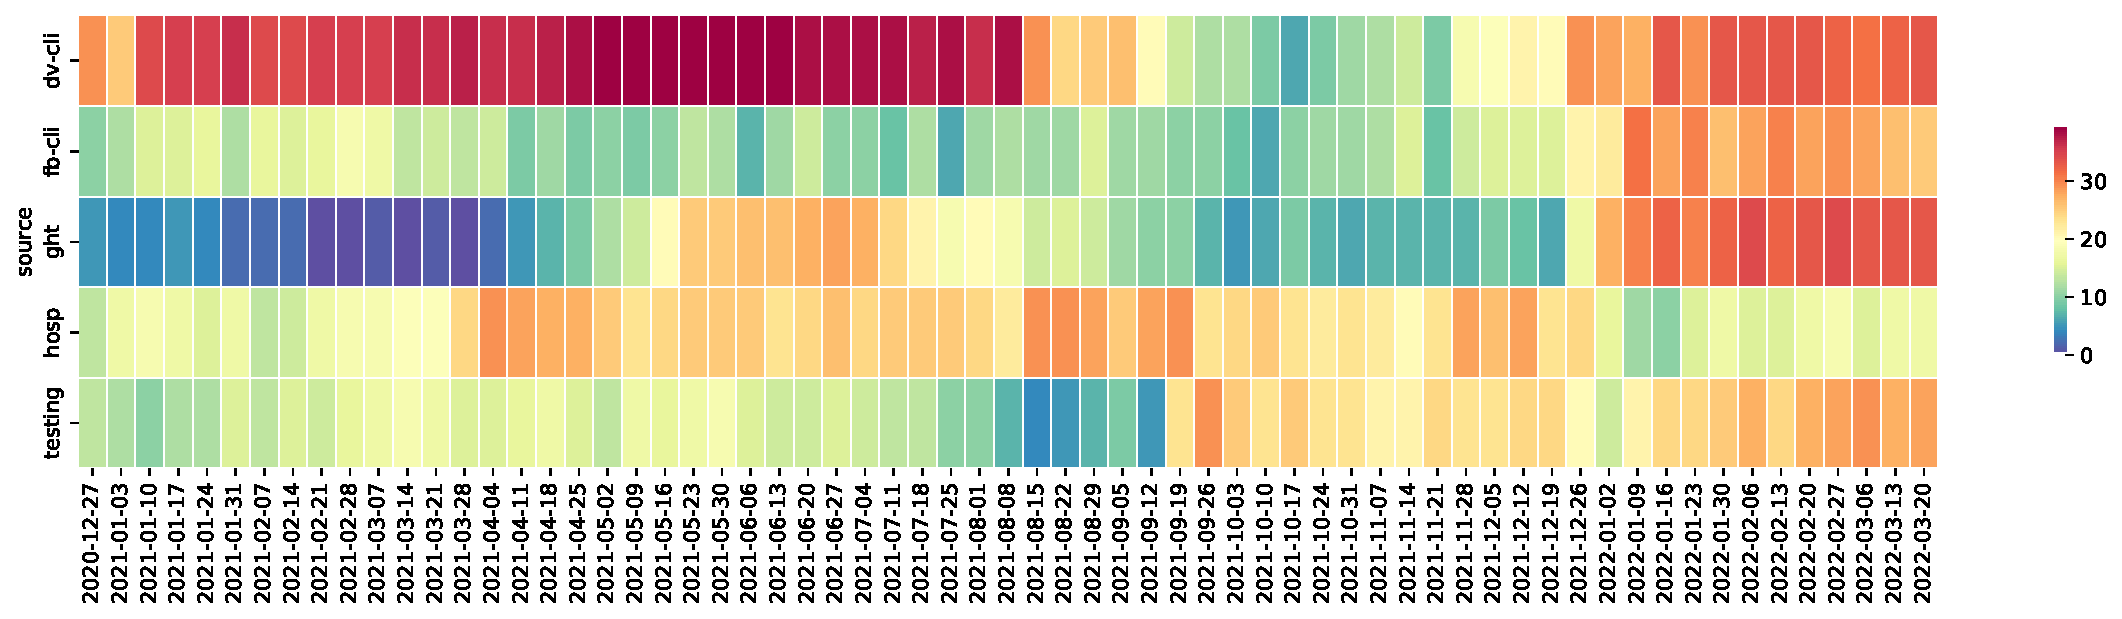
\includegraphics[width=0.99\textwidth]{figs/cases_htmap_te_srcs_len_each_week.pdf}
     \label{fig:TE-surge}
     \caption{Temporal evolution of sources. Heatmap shows the total number of states for which an individual signal was identified as a sources ( signal with significant TE values) for each week. DV-CLI is a source for a significant number of states for a majority of the forecasting weeks.}
     \label{fig:averall_heatmap}
\end{figure*}

\begin{figure*}[!t]
    \centering
    \subfloat[Surge phase]{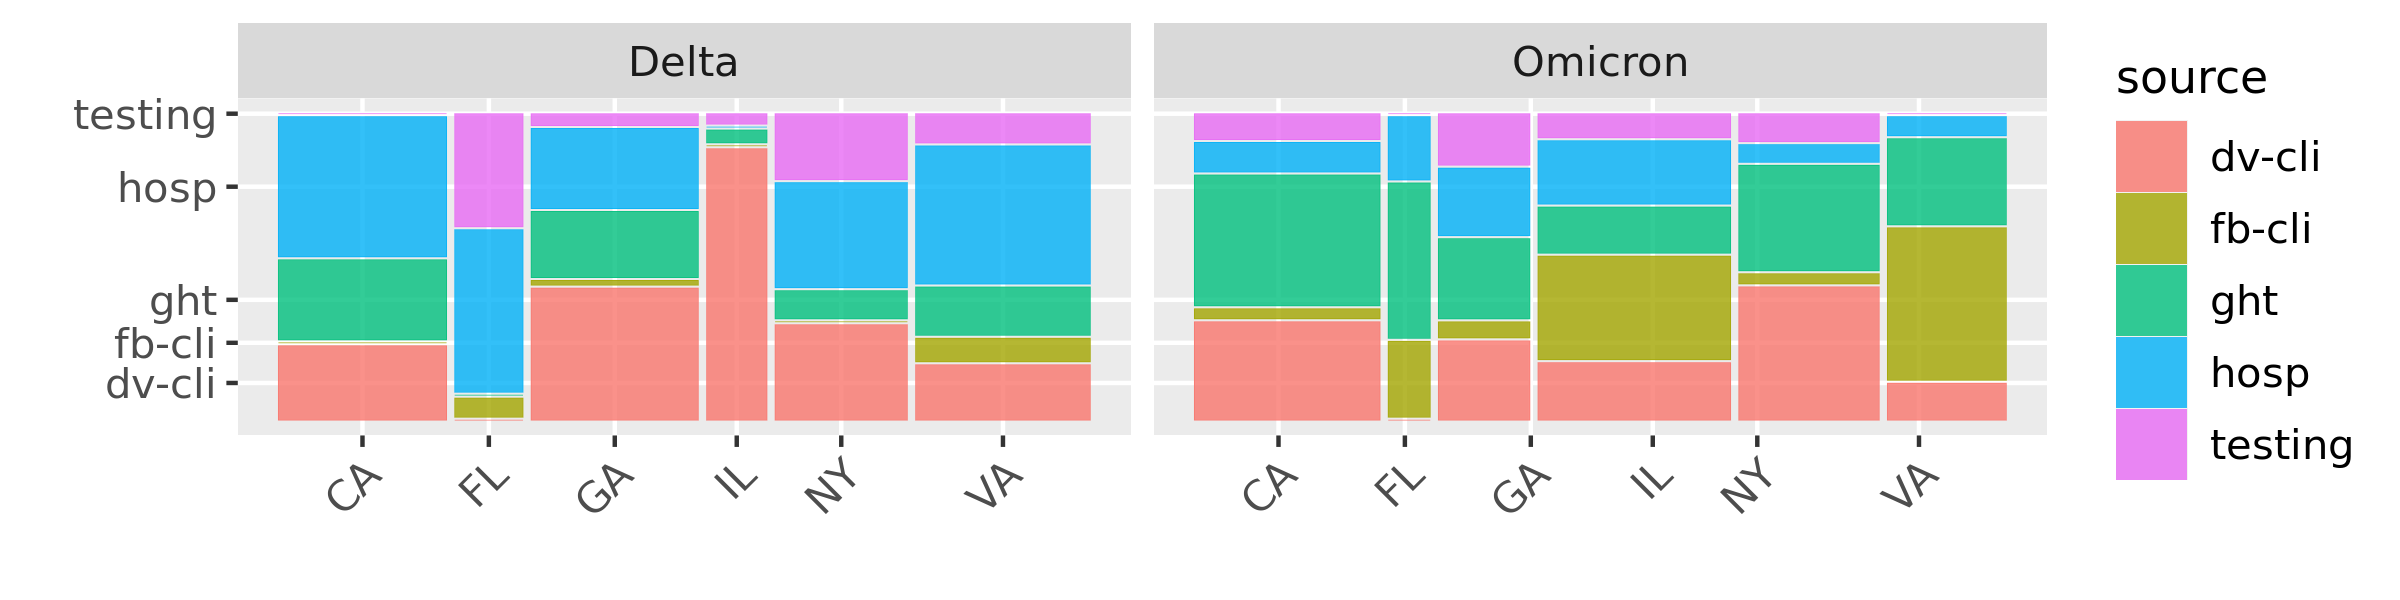
\includegraphics[width=0.99\textwidth]{figs/plot_surge.png}
     \label{Indicators:surge}}
     \hfil
     \subfloat[Overall]{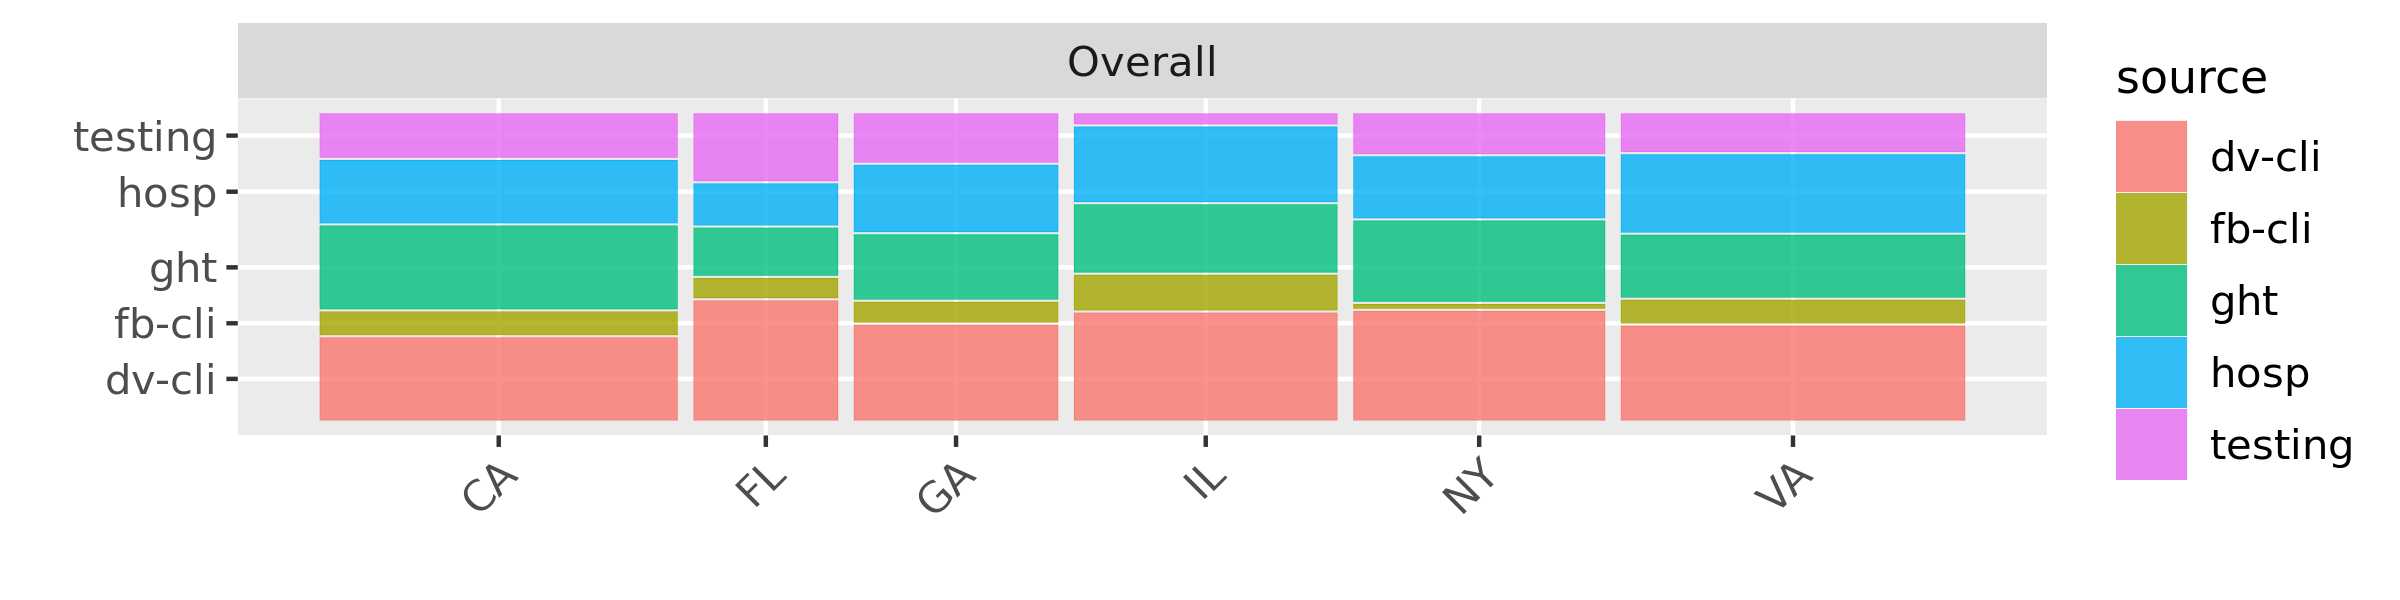
\includegraphics[width=0.99\textwidth]{figs/plot_overall.png}
     \label{Indicators:overall}}
     \caption{Mosaic plot of the leading indicators for selected states during: ~\ref{Indicators:surge} Delta wave (15 July 2021 to 15 August 2021) and  Omicron wave (15 December 2021 to 15 January 2022) and ~\ref{Indicators:overall} overall observed time period i.e. from May 2021 to July 2022. Here the width of a bar denotes the frequency for the overall trends for a state and height of each rectangle within each bar represents the frequency proportion of a specific source.}
 \end{figure*}
 
%     %  \hfil
\begin{figure*}[!t]
    \centering
    \subfloat[TE distribution observed during Surge phase]{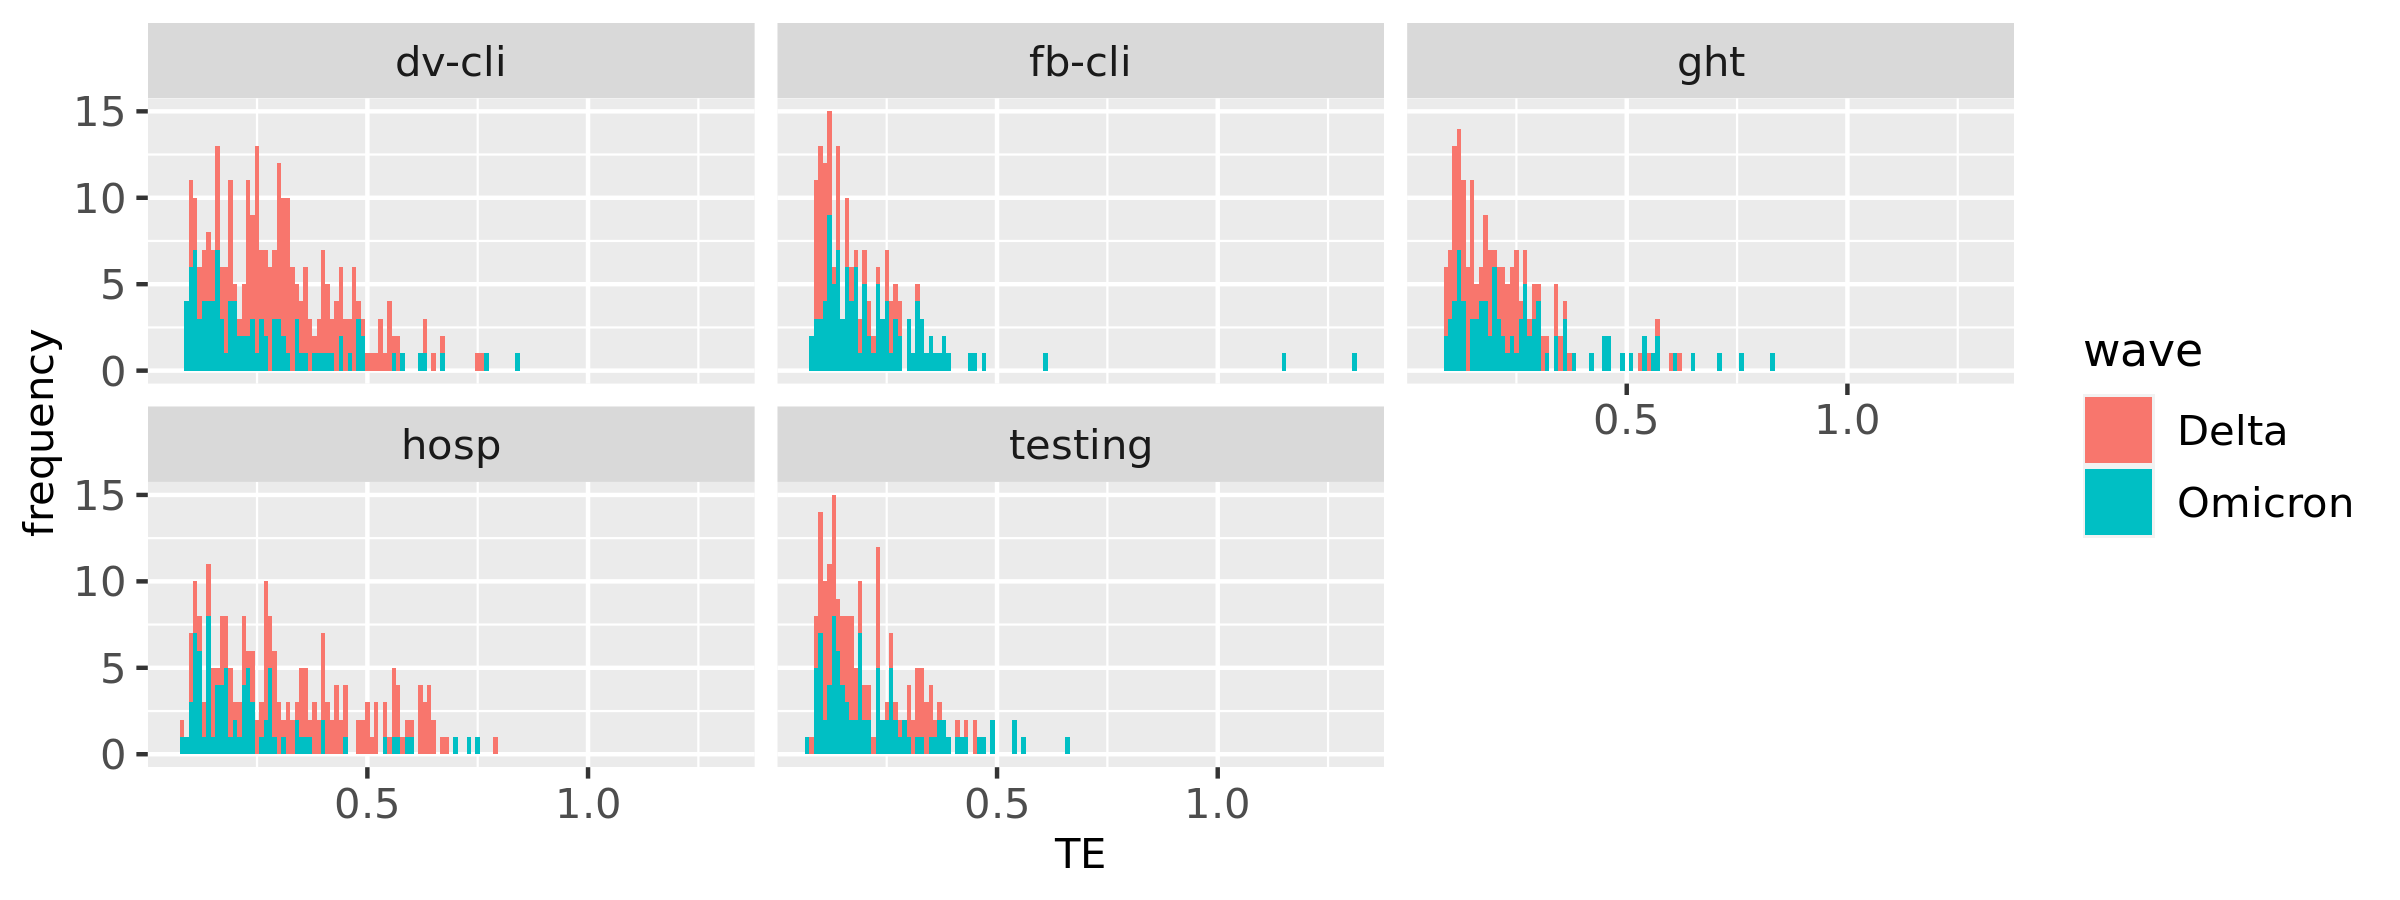
\includegraphics[width=0.99\textwidth]{figs/plot_TE_surge.png}
     \label{fig:TE-surge}}
     \hfil
     \subfloat[Overall observed TE distribution ]{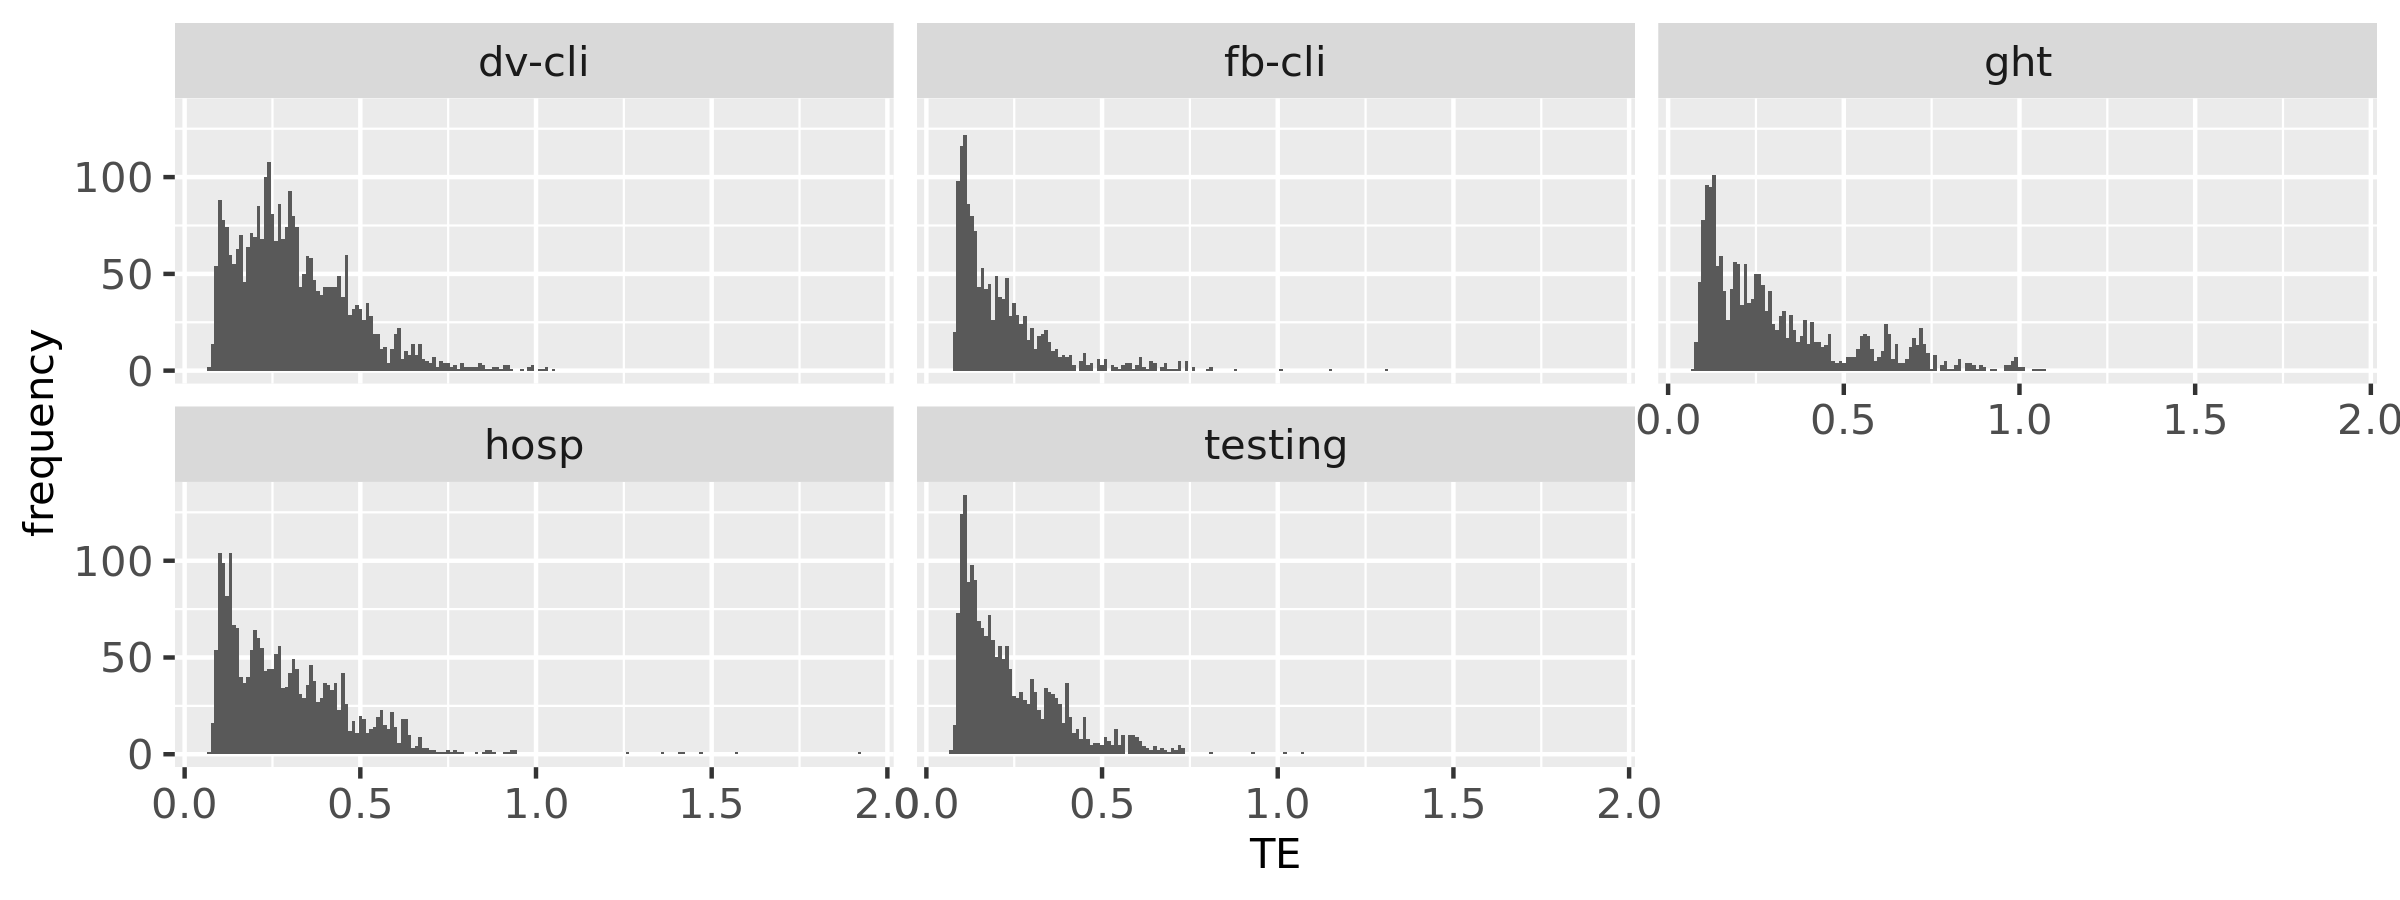
\includegraphics[width=0.99\textwidth]{figs/plot_TE_overall.png}
    \label{fig:TE-overall}}
     \caption{Histogram of the observed transfer entropy (TE) across all states during ~\ref{fig:TE-surge} the Delta and Omicron wave, and ~\ref{fig:TE-overall} overall observed time period.  }
 \end{figure*}

% % \begin{figure*}[ht!]
% %     \centering
% %     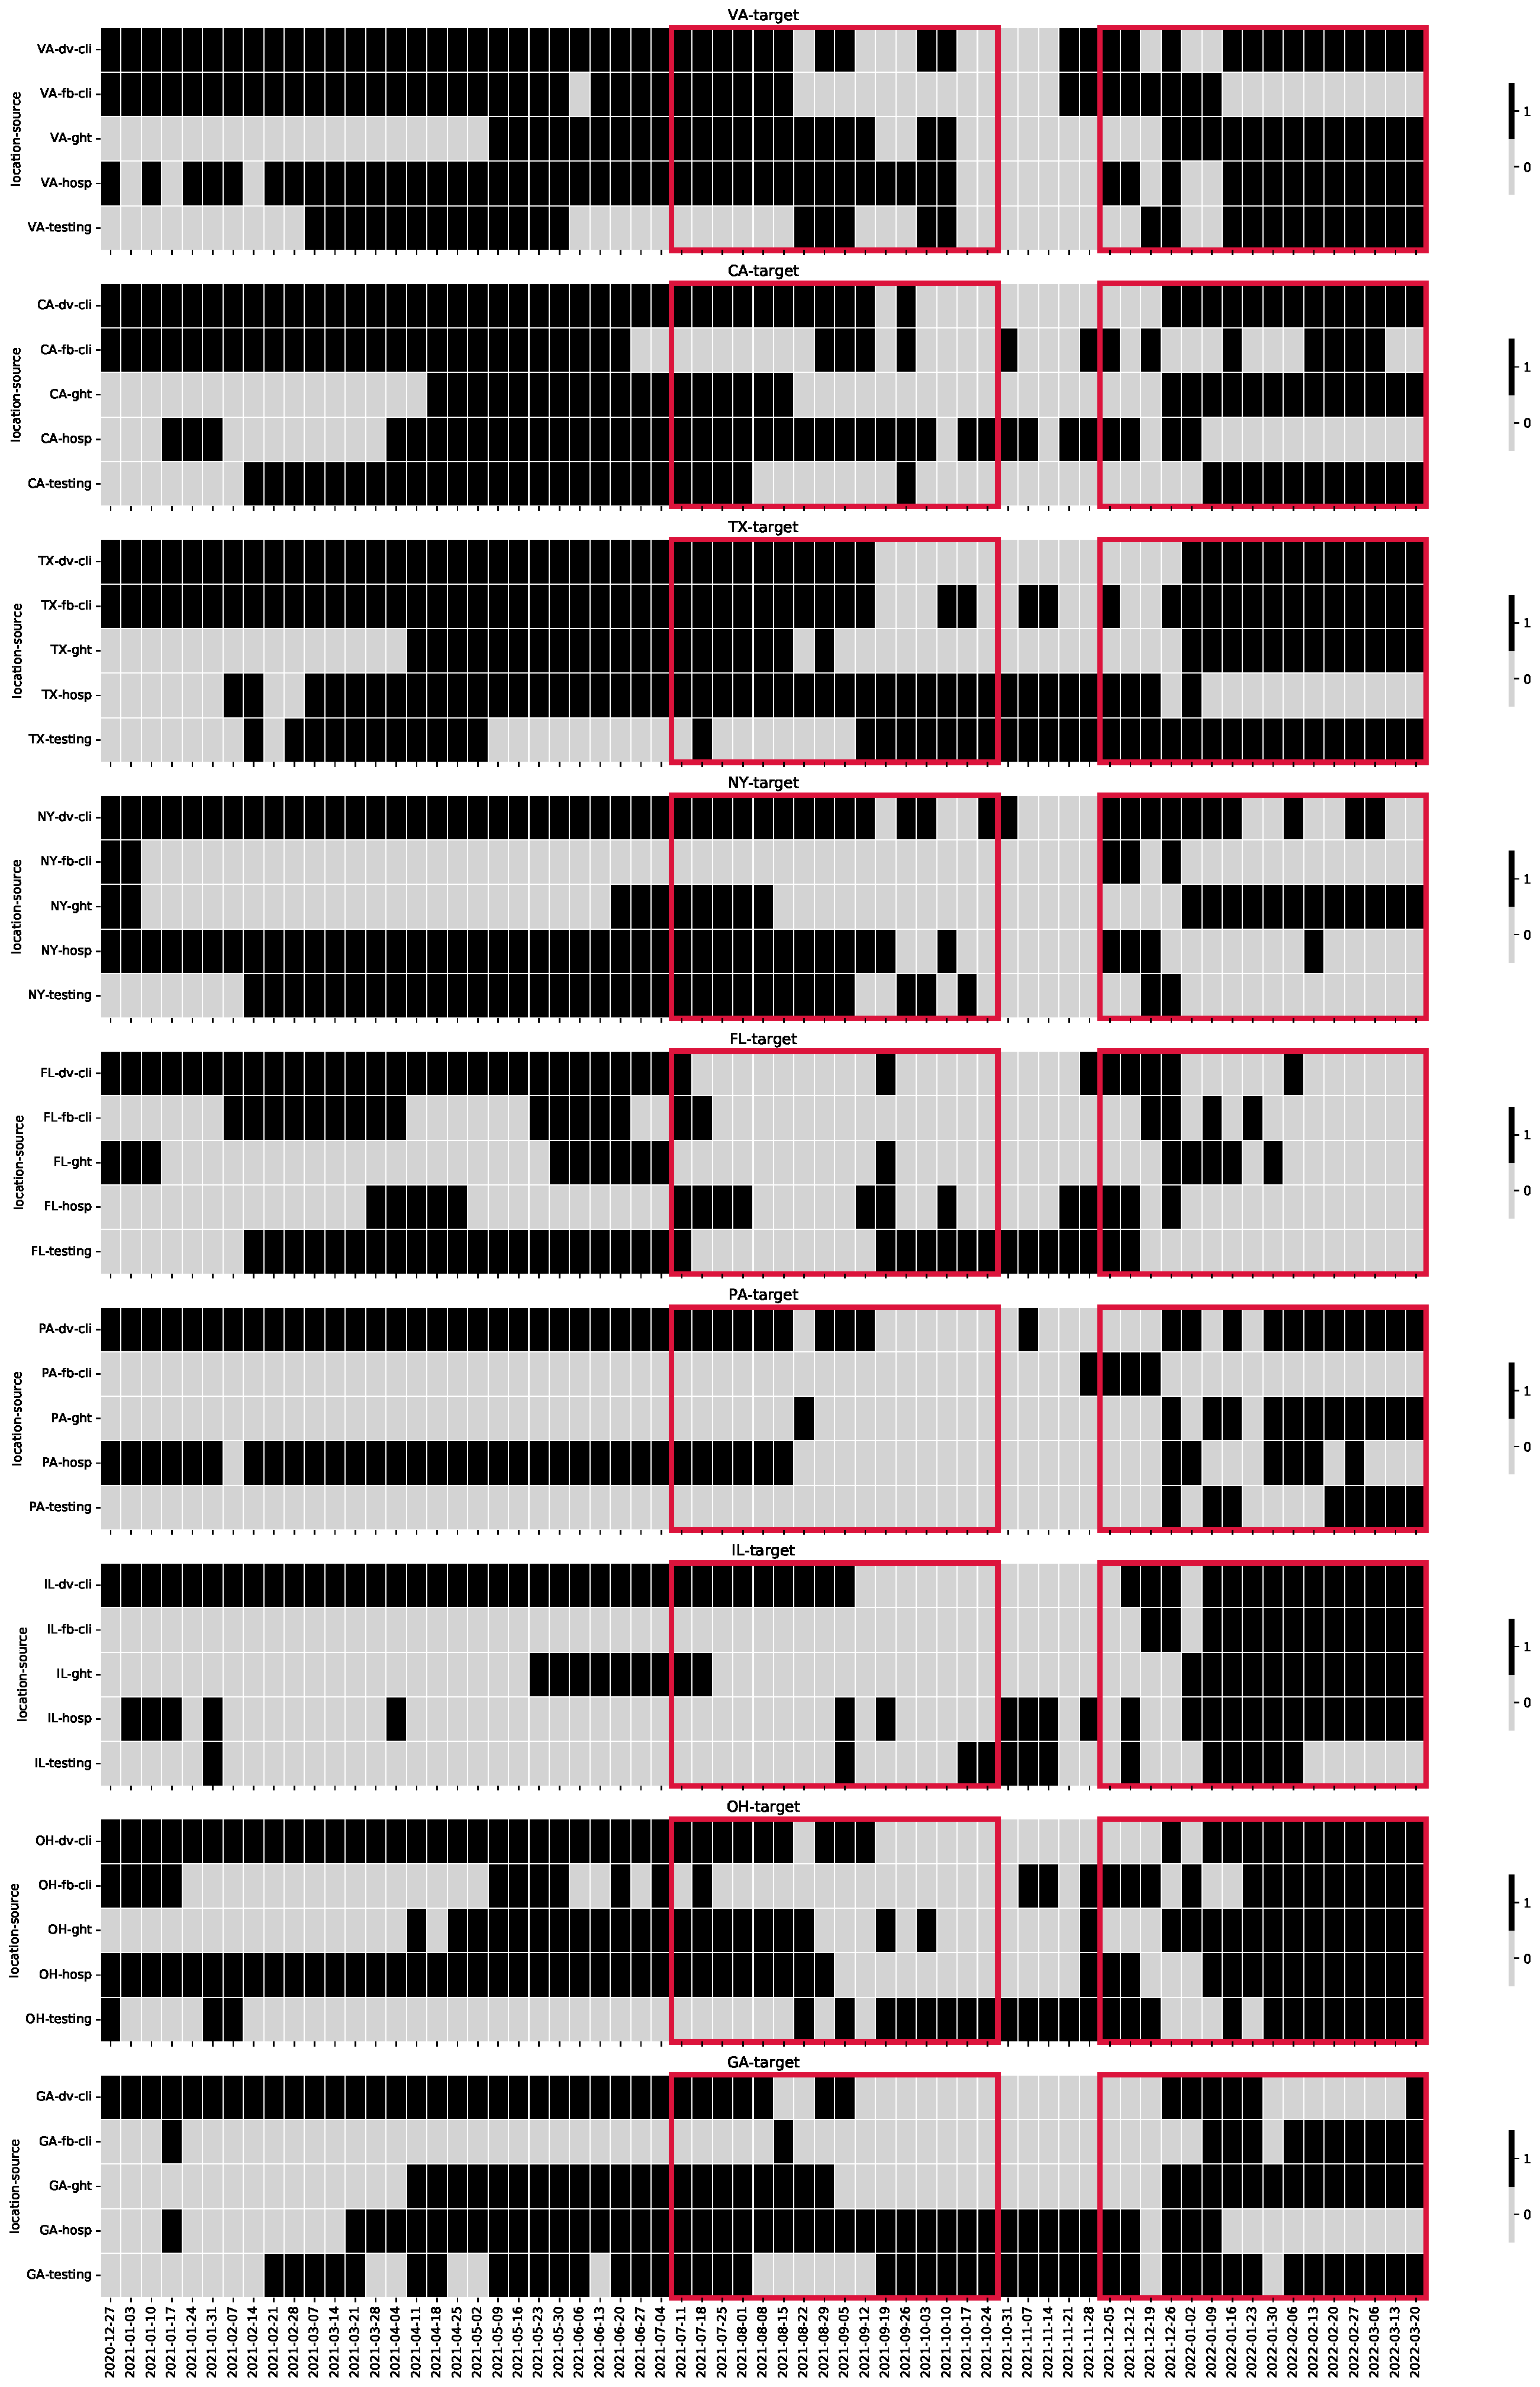
\includegraphics[width=0.8\textwidth]{figs/cases_st_htmap_te_srcs_len_all (1).pdf}
% %     \caption{Data sources for various states across forecast weeks with significant transfer entropy with cases.}
% %     \label{TE-src}
% \end{figure*}

\subsubsection{Phase inference and Prediction} \label{phase:classification}
Once the indicators are obtained, we segment the cases and the indicator time series into different phases. Despite heterogeneity in the COVID-19 time series, we  broadly observe three phases and classify the observed time period based on the rate of change of reported cases: Surge (period of steep growth in cases), Decline, and Plateau. The primary purpose of phase classification is to capture distinct trends in the time series and leverage that information to better train the BMA model. We want to note that the definitions of phases are subjective (several exist\footnote{https://www.cdc.gov/flu/pandemic-resources/planning-preparedness/global-planning-508.html}) and can be user annotated or obtained through standard time-series change point detection algorithms~\cite{aminikhanghahi2017survey}.  

We first approximate the nonlinear time series with a piece-wise linear function. We use a standard R package \verb|segmented| \cite{Rsegmented} to estimate multiple break-points. Note that, in real-time forecasting, since we obtain a new data point each week, the phase segments have to be re-estimated each week. Given the new data point, we would want to refine our estimates of phases. In order to ensure that all of the historical phase estimates do not change, we apply the segmentation each week on data starting from the most recent two break points. The algorithm is described in Algorithm~\ref{alg:rec:piece-fit}.

\begin{algorithm}[ht!]
\footnotesize
\caption{Piece-wise linear fit}
\label{alg:algorithm}
\textbf{Input}: Ground truth $y(1), \dots, y(T)$\\
\textbf{Output}:  Piece-wise linear version of $y(1), \dots, y(T)$ and set of break points $\{b_1, \dots, b_{m}\}$ 
\begin{algorithmic}[1] %[1] enables line numbers
\STATE  Start with $t_0=15$ 
\STATE Get a piece-wise fit for $y(1), y(2), \dots, y(t_0)$ with break points $1
\leq b_1^{(t_0)} \leq \dots\leq  b_{k_{t_0}}^{(t_0)}$
\STATE  $\mathcal{B}(t_0) \gets \{1, b_1^{(t_0)}, \dots, b_{k_{t_0}}^{(t_0)} \}$
\WHILE{$ t_0+1\leq t \leq T$}
\STATE Get a piece-wise fit for $\{y_s : b_{k_{t-1}-2}^{(t-1)}\leq s \leq t\}$
with break points $1 \leq b_1^{(t)}\leq b_2^{(t)}\leq  \dots\leq  b_{k_t}^{(t)}$
\STATE $b^\star_{1} \gets \max \mathcal{B}(t-1)$, $b^\star_{2} \gets\max \mathcal{B}(t-1) \setminus b^\star_{1}$
\STATE $\mathcal{B}(t)\gets (\mathcal{B}(t-1) \setminus \{b^\star_{1} , b^\star_{2}\}) \cup \{1,  b_1^{(t)},\dots, b_{k_t}^{(t)} \}$
\ENDWHILE
\STATE Let $\mathcal{B}(t) = \{ b_1, \dots, b_m \}$ and $b_0=1$ 
\FOR {$0\leq i <m$}
    \STATE $\{\tilde y(t);  b_i \leq t\leq b_{i+1}\}$ is the  linearly interpolation between  $y(b_i)$ and  $y(b_{i+1})$
    \ENDFOR
\STATE \textbf{return}  $\tilde y(1), \dots \tilde y(T)$ and breakpoints set $\{b_1, \dots, b_m\}$
\end{algorithmic}
\label{alg:rec:piece-fit}
\end{algorithm}

Using the estimated break points $\{b_1, \dots, b_m\}$ with Algorithm~\ref{alg:rec:piece-fit} for the ground truth $y_1, \dots, y_t$, we classify the time interval between any two consecutive break-points as a Surge (S), Decline (D), or Plateau (P) phase. We employ a simple criterion for the phase classification, which defines a time interval $(b_k, b_{k+1}]$ as surge  (or decline) phase if there is at least a $10\%$ increment (or at least a $10\%$ reduction) in the case count from the start of the time interval $b_k$ to end of the interval $b_{k+1}$ and plateau phase otherwise.
Let $P(t)$ and $P_1(t),\dots, P_m(t)$, be the phase time series for the piece-wise constant versions (as defined in Algorithm~\ref{alg:rec:piece-fit}) of $Y(t)$ and $X_1(t), \dots, X_m(t)$ respectively. The algorithm to obtain the phase time series for a given time series is described in Algorithm~\ref{alg:phase}. 

Let $ P^{(k)}(t) = (P(t), \dots, P(t-k+1))$ and $P^{(k)}_i(t) =\left(P_i(t), \dots, P_i(t-k+1)\right)$,  then we assume that $P(t)$ is a Markov process that depends only on   $\Paux(t-1) = \{\tilde P_i(t-1); i\in \Lambda(t)\}$ and $ P^{(\tau)}(t-1)$, where $\tau =\max_i \tau_i$. That is, the phase at time $t$ for the case count time series $P(t)$ can be written as a function of past $\tau$ values of itself and past $\tau_i$ phases of the $X_i$ when $i$ is restricted to the leading indicators set $\Lambda(t)$. Thus we have 
\begin{equation}
    P(t) = f\big( P^{(\tau)}(t-1), \Paux(t-1) \big),
\end{equation}
where $f$ is a $ \{S, D, P\} $ valued random function such that for a given phase sequence at time $t-1$,  $P^{(\tau)}(t-1) = w$ and $ P^{(\tau_i)}_i(t-1) =w_i$ 
\begin{align*}
    f(w, w_1, \dots, w_m) 
    &= \begin{cases}
    S & \text{w.p. } p_1(t) \\
    D& \text{w.p. } 1-p_0(t)-p_1(t)\\
    P& \text{w.p. } p_0(t) 
    \end{cases}
\end{align*}
where the probabilities $p_0(t)$ and $ p_1(t)$ are estimated empirically at every time $t$ as
{\footnotesize
\begin{align*}
    &\hat{p}_1(t) \\
    & =\frac{ |\{P(t) = S\}\cap \{P^{(\tau)}(t-1) =w, P^{(\tau_i)}_i(t-1) =w_i;i\in \Lambda(t)\} |} {| \{P^{(\tau)}(t-1) =w, P^{(\tau_i)}_i(t-1) =w_i;i\in \Lambda(t)\} |}
\end{align*} }
and 
{\footnotesize
\begin{align*}
    &\hat{p}_0(t) \\
    & =\frac{ |\{P(t) = P\}\cap \{P^{(\tau)}(t-1) =w, P^{(\tau_i)}_i(t-1) =w_i;i\in \Lambda(t)\} |} {| \{P^{(\tau)}(t-1) =w, P^{(\tau_i)}_i(t-1) =w_i;i\in \Lambda(t)\} |}.
\end{align*} }

As an example, suppose we obtain a subset of signals $\{1,2,5\}$ as the leading indicators with lags $\{\tau_1=2, \tau_2=1, \tau_5=1\}$. Since the maximum lag is 2, $\tau=2$. Thus $\tilde P(t) = (P(t-1), P(t-2))$, $\Paux(t) = (P_1(t-1), P_1(t-2), P_2(t-1), P_5(t-1))$. 
Now, the vector $\mathbf{w}=(w, w_1, w_2, w_5)=[P(t-1), P(t-2), P_1(t-1), P_1(t-2), P_2(t-1), P_5(t-1)]$. In Figure~\ref{fig:seq_ex}, we illustrate the process of predicting the phase. 
\begin{figure*}
    \centering
    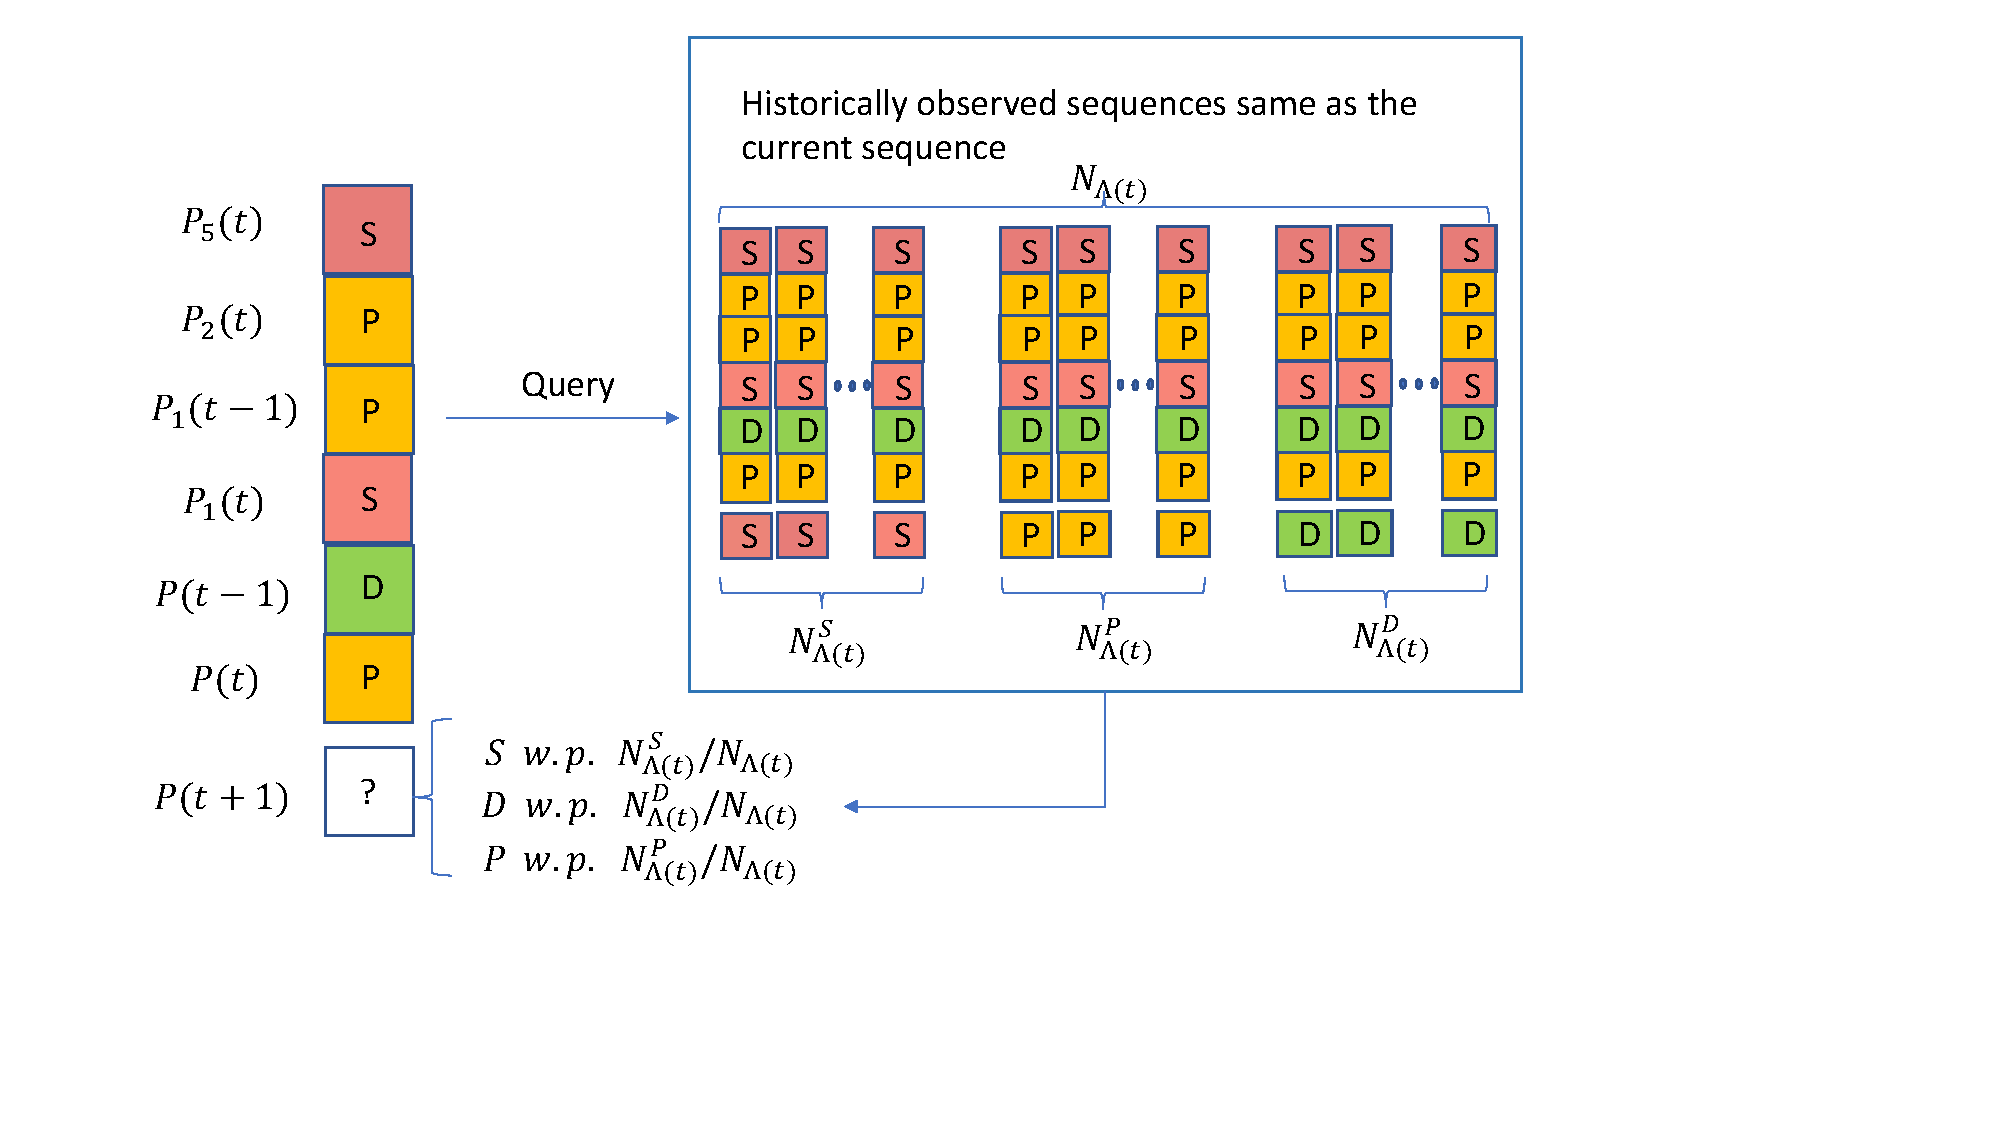
\includegraphics[width=.75\textwidth]{PI-BMA-IEEE-BigData2022_extended/figs/seq_freq_algo.pdf}
    \caption{An example of phase prediction.}
    \label{fig:seq_ex}
\end{figure*}








% \begin{figure*}[ht!]
%     \centering
%     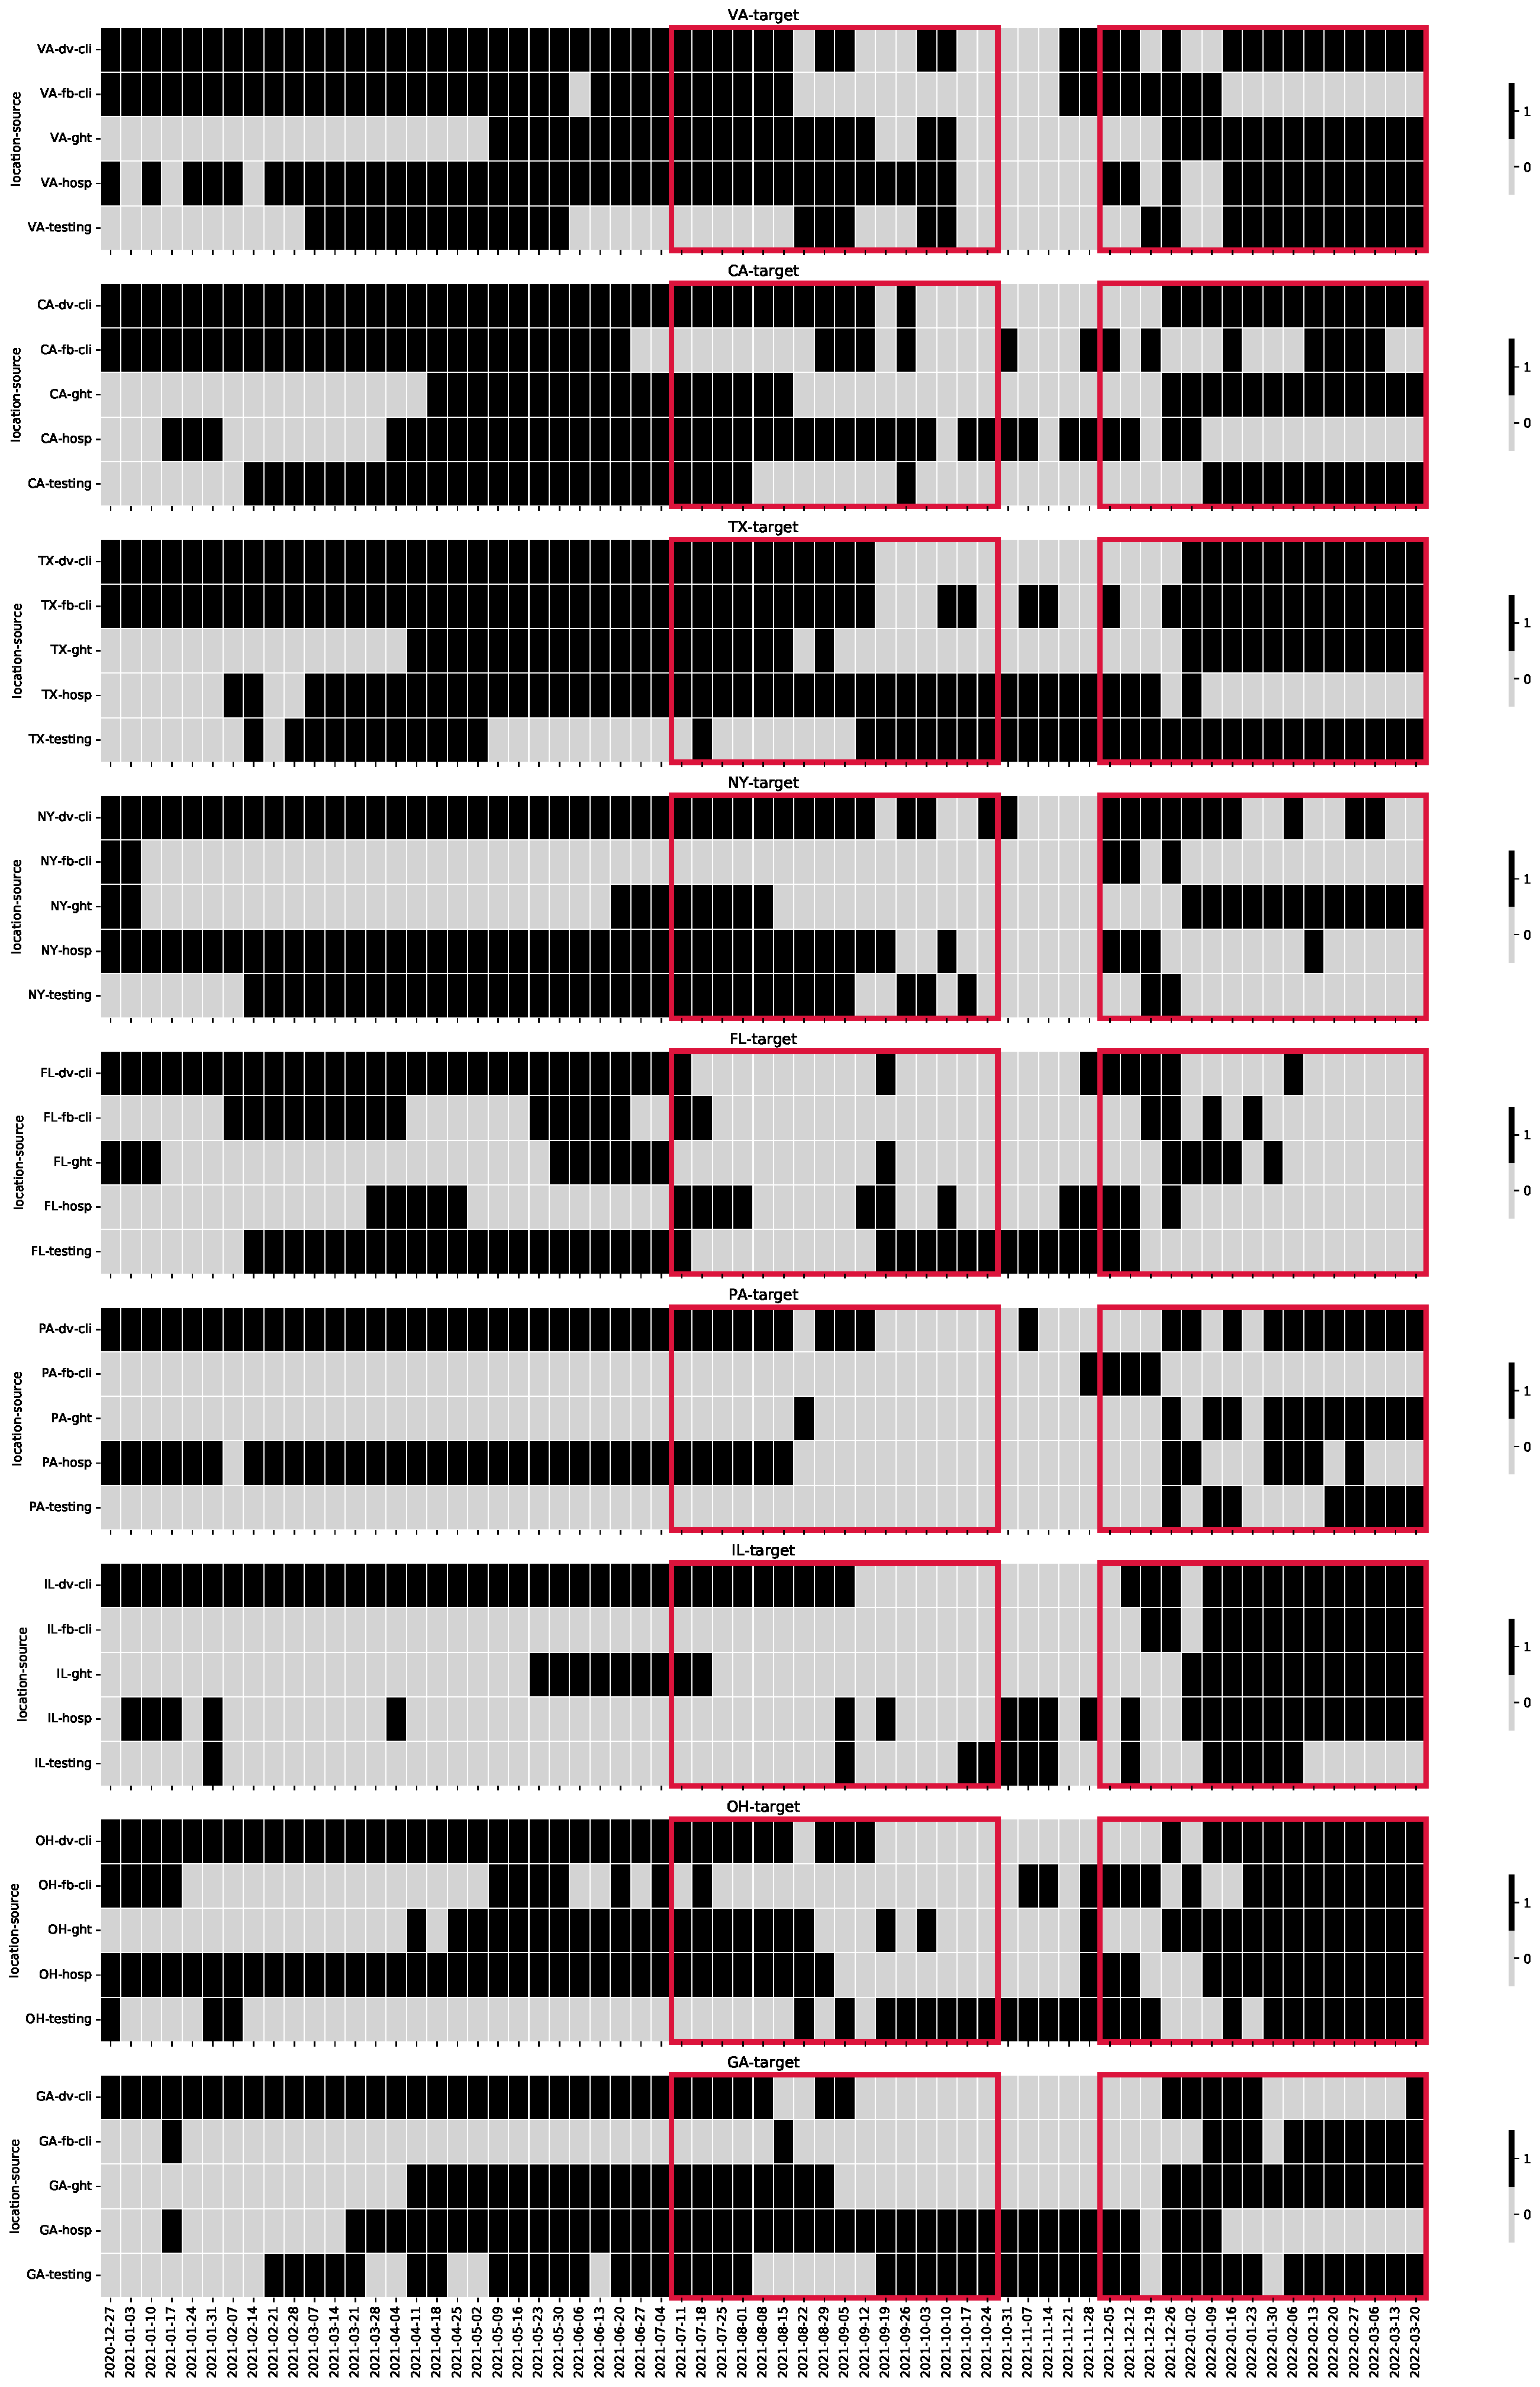
\includegraphics[width=0.8\textwidth]{figs/cases_st_htmap_te_srcs_len_all (1).pdf}
%     \caption{Data sources for various states across forecast weeks with significant transfer entropy with cases.}
%     \label{TE-src}
% \end{figure*}


\begin{algorithm}[!t]
\caption{Transfer Entropy}
\label{alg:TE}
\textbf{Input}:  Auxiliary sources $\Lambda =\{1, \dots, m\}.$\\
Observed target case count time series $y(t)$.\\
Observed source time series $x_i(t)$, for each $i\in\Lambda$.\\
\textbf{Output}: Probabilistic estimate of $P(t+1)$\\
\begin{algorithmic}[1]
\STATE Obtain phase time series  $P(t), P_1(t), \dots P_m(t)$ from Algorithm~\ref{alg:phase} for $y, x_1, \dots, x_m$.
\STATE Compute $h_i = \mathsf{TE}_{X_i\to Y}$ for each pair $(X_i, Y)$ with appropriate order $\tau_i$.
\STATE Obtain $\Lambda(t)$ using Python package \verb|IDTxL|.
  \STATE $\tau \gets \max_{i\in\Lambda(t)} \tau_i$\\
  $\tilde P(t) := (P(t), P(t-1), P(t-\tau+1))$
  \FOR{$i \in \Lambda(t)$}
  \STATE $\tilde P_i(t) := (P_i(t), P_i(t-1), \dots,  P_i(t-\tau_i+1))$
  \ENDFOR
  \STATE Given  $\tilde P_i(t) = w_i$ \\
  $n_o \gets |\{\tilde P_i(s) =  w_i;~ i\in \Lambda(t), 1\leq s\leq t-1\}|$
\IF{$\Lambda(t) =\emptyset$ or $n_o=0$}
    \STATE $P(t+1) \gets P(t)$
  \ELSE
    \WHILE{$n_o/t \leq  0.1$}
    \STATE update $\Lambda(t) \gets \Lambda(t)\setminus \{j: h_j = \min_{i\in \Lambda(t)} h_i\}$
  \ENDWHILE
    \STATE $P(t+1) \gets f(\tilde P(t), \tilde P_i(t)) $
  \ENDIF
 \STATE \textbf{return}  $(\hat p_1(t), \hat p_0(t)) $
\end{algorithmic}
\end{algorithm}


\begin{algorithm}[ht]
\caption{Phase classification}
\label{alg:phase}
\textbf{Input}:  Time series $y(t)$.\\
\textbf{Output}:  Phase time series  $P(t)$.\\
\textbf{Parameters}: $\delta$
\begin{algorithmic}[1]
\STATE Approximate $y(t)$ with a piece-wise linear time series $\tilde y(t)$ with breakpoints $b_1, \dots b_n$
\IF{$y_{b_{i+1}} > (1+\delta)  y_{b_i}$} 
    \STATE $P(t) \gets S$ for $t\in (b_i, b_{i+1}]$
  \ELSE \IF{$y_{b_{i+1}} < (1-\delta) y_{b_i}$}
    \STATE $P(t) \gets D$ for $t\in (b_i, b_{i+1}]$
    \ELSE 
    \STATE $P(t) \gets P$
  \ENDIF
      \ENDIF
\end{algorithmic}
\end{algorithm}


\section{Results}
\begin{figure}[ht!]
    \centering
    % \begin{subfigure}{.4\textwidth}
    % %\includegraphics[width=.45\linewidth]{figs/overall_perf_BMA_v3.pdf}
    % 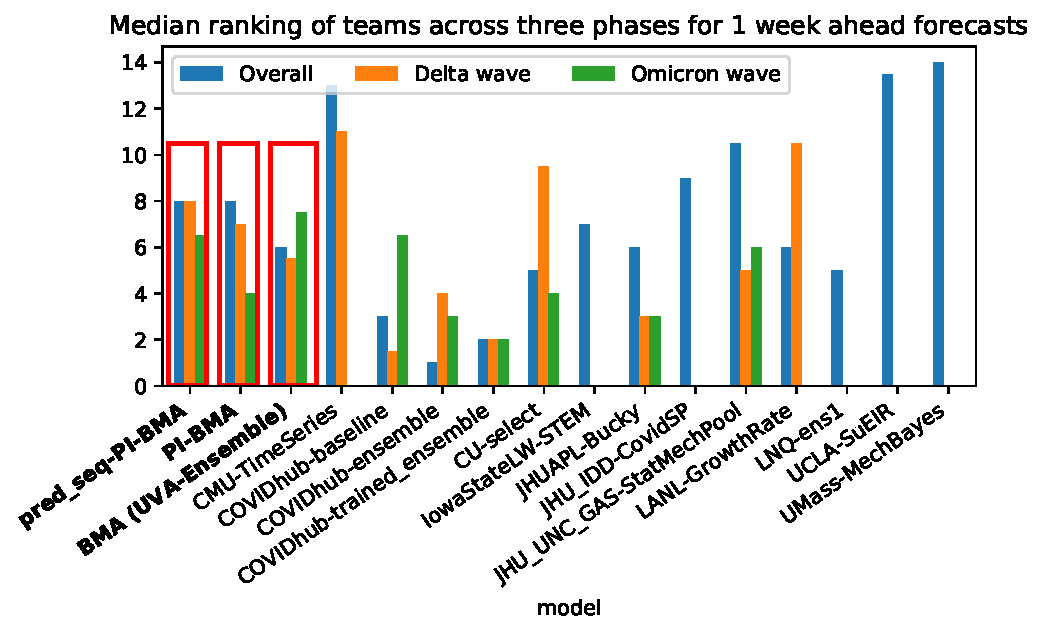
\includegraphics[width=.99\textwidth]{figs/pred_PI_BMA_1_wk_median_rank_various_weeks_seq.pdf}
    % \caption{1 week ahead}
    % \label{fig:1wk_ranking}
    % \end{subfigure}
    \begin{subfigure}{.5\textwidth}
    %\includegraphics[width=.45\linewidth]{figs/overall_perf_BMA_v3.pdf}
    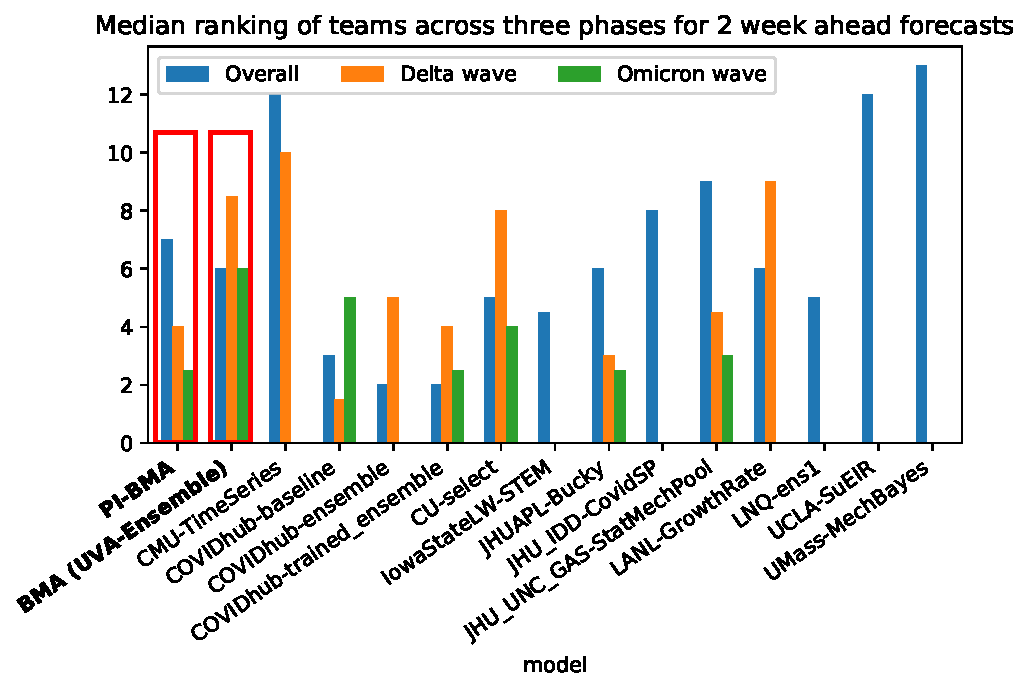
\includegraphics[width=.99\textwidth]{figs/pred_PI_BMA_2_wk_median_rank_various_weeks_seq_v2.pdf}
    \caption{2 week ahead}
    \label{fig:2wk_ranking}
    \end{subfigure}
    % \begin{subfigure}{.4\textwidth}
    % %\includegraphics[width=.45\linewidth]{figs/overall_perf_BMA_v3.pdf}
    % 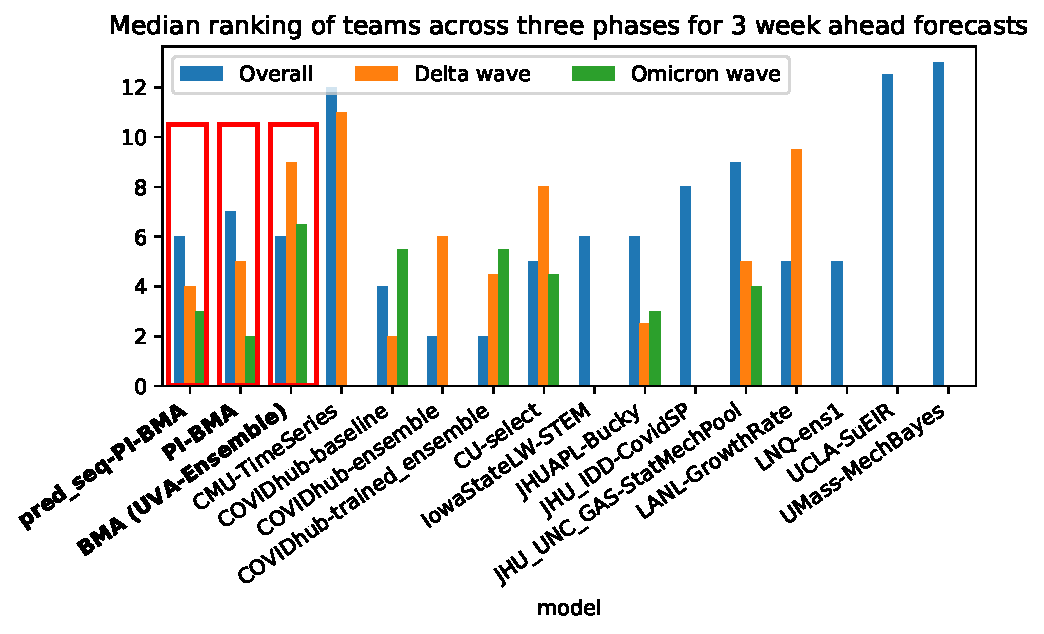
\includegraphics[width=.99\textwidth]{figs/pred_PI_BMA_3_wk_median_rank_various_weeks_seq.pdf}
    % \caption{3 week ahead}
    % \label{fig:3wk_ranking}
    % \end{subfigure}
    \begin{subfigure}{.5\textwidth}
      %\includegraphics[width=.45\linewidth]
              %{figs/median_bma_methods_1_week_ahead.pdf}
      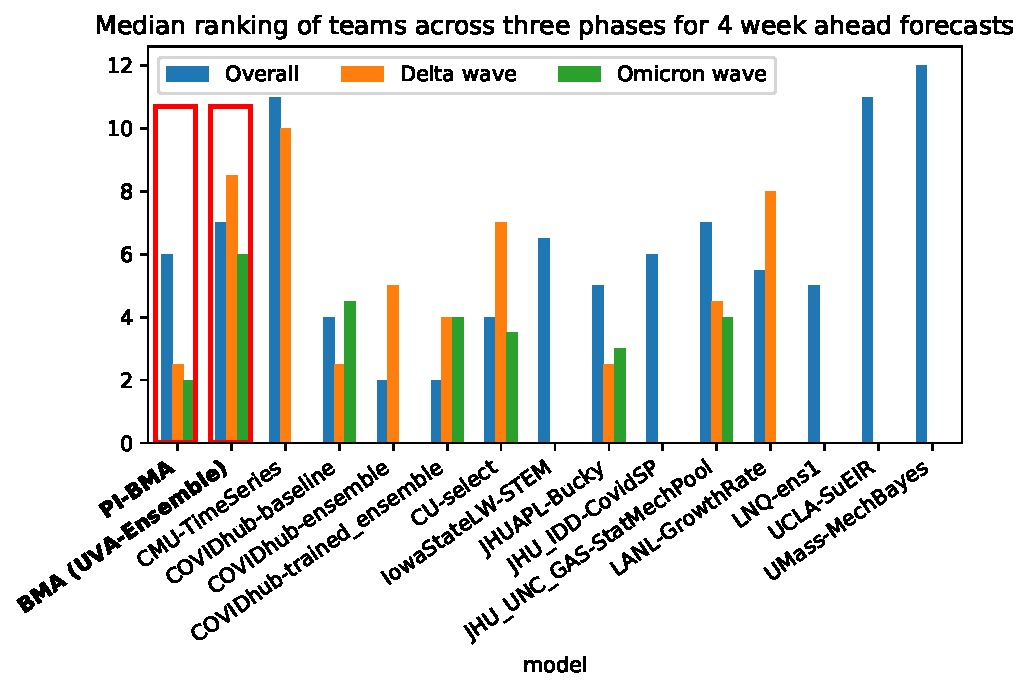
\includegraphics[width=.99\textwidth]{figs/pred_PI_BMA_4_wk_median_rank_various_weeks_seq_v2.pdf}
      \caption{4 week ahead}
      \label{fig:4wk_ranking}
     
    \end{subfigure}
        \caption{A comparison of several \hub{} models performance. The median ranking of models for 2 and 4 week ahead forecasts in (a) and (d) computed across different regimes, respectively. Blue bars shows the median ranking of models computed across all the forecasting weeks, orange bars correspond to the median ranking of models computed for the Delta wave's surge phase, and green bars correspond to the median ranking of models during the Omicron wave's surge phase. \textbf{The rankings across different phases indicate that the PI-BMA (red box) is able to provide significantly better forecasts that our UVA-Ensemble model, especially 4 weeks ahead, for critical surge phases corresponding to the \emph{Delta wave} (\textbf{median ranking of 2}) and the \emph{Omicron wave} (\textbf{median ranking of 2})}.  }
\label{fig:match_frac}
\end{figure}
In all our analysis, we consider aggregate performance across three regimes, ($i$) Overall$-$80 forecasts weeks (1 August, 2020 $-$ 1 January, 2022), ($ii$) Delta wave surge region (15 July 2021 $-$ 15 August 2021), and ($iii$) Omicron wave (15 December, 2021 $-$ 15 January 2022). The latter two regimes are specifically considered as these correspond to the surge phases where most models failed to forecast the rapid increase in cases \cite{ray2021challenges}.
\subsection{Retrospective Evaluation: A Comparison with \hub{} Models}\label{sec:comp_hub}
Since early 2020, over 100 models from dozens of teams have submitted forecasts to \hub{}, with the numbers varying each week. The model details are available in \cite{COVID-Hub}. Among the several teams, only a handful have provided forecasts consistently, especially at the county level. As a fair comparison, we only consider teams that have been providing consistent forecasts across most counties and targets since August 2020. It should be noted that across the 80 forecasting weeks, 15 models have provided a significant number of forecasts. As the pandemic progressed, we observed that the number of models started to drop after July 2021. The teams provide probabilistic forecasts in the quantile format. To compare the forecast quantiles of the different models, we use the Weighted Interval Score (WIS), the \emph{de facto} standard in the epidemiological forecasting community for probabilistic forecast evaluation \cite{bracher2020evaluating}:
\begin{align}
    WIS_{\alpha_{0:k}} (F,y) = \frac{1}{K+0.5} \sum_{k=0}^{K} \frac{\alpha_k}{2} (u_k-l_k) + \nonumber\\ \frac{2}{\alpha_k} (l_k-y) \mathbbm{1}(y<l_k) + \frac{2}{\alpha_k} (y-u_k) \mathbbm{1}(y>u_k)
    \label{eq:wis}
\end{align}
where $y$ is the observed value (ground truth case count corresponding to a week) for a given location and date, $F$ is the forecast defined in terms of the median $m$, upper quantiles $u_k$ and lower quantiles $l_k$ of the predictive distribution, respectively. $K=3$ is the number of intervals considered. 

The model performances are first ranked for each forecast week and target horizon by considering its median WIS score across all the counties (model having the lowest median score is ranked one). We next determine the median ranking of different models during different regimes, and the results are shown in Figures~\ref{fig:2wk_ranking} and~\ref{fig:4wk_ranking} for 2 weeks ahead and 4 weeks ahead forecast horizons, respectively. The blue bars, which corresponds to the median ranking computed across all forecasting weeks, indicate that both BMA (UVA-Ensemble) and PI-BMA are ranked around 6$-$7. \textbf{Focusing on the more challenging target of 4-weeks ahead (since the uncertainty is higher), we observe that the PI-BMA is one the top-ranked models during the critical phases of Delta wave surge (median ranking of 2 out of 9) and Omicron wave surge (median ranking of 2 out of 6). The PI-BMA's performance indicates that the model is able to effectively incorporate the phase information and provide considerably better forecasts during critical phases when compared to both BMA (UVA-Ensemble) and the rest of the forecast hub models. It should be noted that, the \emph{COVIDhub ensemble} and \emph{COVIDhub-trained\_ensemble} use forecasts from highly tuned individual models but our model is able to out perform them during the critical phases. This validates the use of selective sampling of training data by ensembling methods}. 
% An example of a floating figure using the graphicx package.
% Note that \label must occur AFTER (or within) \caption.
% For figures, \caption should occur after the \includegraphics.
% Note that IEEEtran v1.7 and later has special internal code that
% is designed to preserve the operation of \label within \caption
% even when the captionsoff option is in effect. However, because
% of issues like this, it may be the safest practice to put all your
% \label just after \caption rather than within \caption{}.
%
% Reminder: the "draftcls" or "draftclsnofoot", not "draft", class
% option should be used if it is desired that the figures are to be
% displayed while in draft mode.
%
%\begin{figure}[!t]
%\centering
%\includegraphics[width=2.5in]{myfigure}
% where an .eps filename suffix will be assumed under latex, 
% and a .pdf suffix will be assumed for pdflatex; or what has been declared
% via \DeclareGraphicsExtensions.
%\caption{Simulation results for the network.}
%\label{fig_sim}
%\end{figure}

% Note that the IEEE typically puts floats only at the top, even when this
% results in a large percentage of a column being occupied by floats.


% An example of a double column floating figure using two subfigures.
% (The subfig.sty package must be loaded for this to work.)
% The subfigure \label commands are set within each subfloat command,
% and the \label for the overall figure must come after \caption.
% \hfil is used as a separator to get equal spacing.
% Watch out that the combined width of all the subfigures on a 
% line do not exceed the text width or a line break will occur.
%
%\begin{figure*}[!t]
%\centering
%\subfloat[Case I]{\includegraphics[width=2.5in]{box}%
%\label{fig_first_case}}
%\hfil
%\subfloat[Case II]{\includegraphics[width=2.5in]{box}%
%\label{fig_second_case}}
%\caption{Simulation results for the network.}
%\label{fig_sim}
%\end{figure*}
%
% Note that often IEEE papers with subfigures do not employ subfigure
% captions (using the optional argument to \subfloat[]), but instead will
% reference/describe all of them (a), (b), etc., within the main caption.
% Be aware that for subfig.sty to generate the (a), (b), etc., subfigure
% labels, the optional argument to \subfloat must be present. If a
% subcaption is not desired, just leave its contents blank,
% e.g., \subfloat[].


% An example of a floating table. Note that, for IEEE style tables, the
% \caption command should come BEFORE the table and, given that table
% captions serve much like titles, are usually capitalized except for words
% such as a, an, and, as, at, but, by, for, in, nor, of, on, or, the, to
% and up, which are usually not capitalized unless they are the first or
% last word of the caption. Table text will default to \footnotesize as
% the IEEE normally uses this smaller font for tables.
% The \label must come after \caption as always.
%
%\begin{table}[!t]
%% increase table row spacing, adjust to taste
%\renewcommand{\arraystretch}{1.3}
% if using array.sty, it might be a good idea to tweak the value of
% \extrarowheight as needed to properly center the text within the cells
%\caption{An Example of a Table}
%\label{table_example}
%\centering
%% Some packages, such as MDW tools, offer better commands for making tables
%% than the plain LaTeX2e tabular which is used here.
%\begin{tabular}{|c||c|}
%\hline
%One & Two\\
%\hline
%Three & Four\\
%\hline
%\end{tabular}
%\end{table}


% Note that the IEEE does not put floats in the very first column
% - or typically anywhere on the first page for that matter. Also,
% in-text middle ("here") positioning is typically not used, but it
% is allowed and encouraged for Computer Society conferences (but
% not Computer Society journals). Most IEEE journals/conferences use
% top floats exclusively. 
% Note that, LaTeX2e, unlike IEEE journals/conferences, places
% footnotes above bottom floats. This can be corrected via the
% \fnbelowfloat command of the stfloats package.


\section{Conclusion}
Based on the observations made during the COVID-19 forecasting efforts, this paper proposed a novel phase-based Bayesian model averaging, a modification of the current model. The paper provides three critical contributions, $(i)$ a phase-based sampling approach for training the ensemble, $(ii)$ a novel transfer-entropy-based leading indicator identification method, and $(iii)$ a phase prediction method that uses the phases from the leading indicators to predict the future phase. The performance of the PI-BMA model validates the utility of the  phase-based training methodology. The proposed method is fairly generic and can be incorporated in most ensemble model.

In future work, we plan on exploring other variants of transfer entropy. In addition, several of the auxiliary data sources undergo revision and developing a model to correct for it might improve phase forecasting. An extended version of the manuscript containing additional analysis and results are available at \url{https://github.com/aniruddhadiga/phase-informed-BMA}. 

\section{Acknowlegments}
Funding agencies: NSF Rapid 2142997, CSTE/CDC 5 NU38OT000297, NIH Grant 1R01GM109718, NSF BIG DATA Grant IIS-1633028, NSF Grant No.: OAC-1916805, NSF Expeditions in Computing Grant CCF-1918656, CCF-1917819, NSF RAPID CNS-2028004, NSF RAPID OAC-2027541, US-CDC 75D30119C05935, a grant from Google, UVA Strategic Investment Fund award number SIF160, DTRA under Contract No. HDTRA1-19-D-0007, and VDH Grant VDH-21-501-0141



% conference papers do not normally have an appendix



% % use section* for acknowledgment
% \ifCLASSOPTIONcompsoc
%   % The Computer Society usually uses the plural form
%   \section*{Acknowledgments}
% \else
%   % regular IEEE prefers the singular form
%   \section*{Acknowledgment}
% \fi







% trigger a \newpage just before the given reference
% number - used to balance the columns on the last page
% adjust value as needed - may need to be readjusted if
% the document is modified later
%\IEEEtriggeratref{8}
% The "triggered" command can be changed if desired:
%\IEEEtriggercmd{\enlargethispage{-5in}}

% references section

% can use a bibliography generated by BibTeX as a .bbl file
% BibTeX documentation can be easily obtained at:
% http://mirror.ctan.org/biblio/bibtex/contrib/doc/
% The IEEEtran BibTeX style support page is at:
% http://www.michaelshell.org/tex/ieeetran/bibtex/
\bibliographystyle{IEEEtran}
% argument is your BibTeX string definitions and bibliography database(s)
\bibliography{ref.bib}
%
% <OR> manually copy in the resultant .bbl file
% set second argument of \begin to the number of references
% (used to reserve space for the reference number labels box)
% \begin{thebibliography}{1}

% \bibitem{IEEEhowto:kopka}
% H.~Kopka and P.~W. Daly, \emph{A Guide to \LaTeX}, 3rd~ed.\hskip 1em plus
%   0.5em minus 0.4em\relax Harlow, England: Addison-Wesley, 1999.

% \end{thebibliography}




% that's all folks
\end{document}


